%% 
%% Copyright 2019-2024 Elsevier Ltd
%% 
%% Version 2.4
%% 
%% This file is part of the 'CAS Bundle'.
%% --------------------------------------
%% 
%% It may be distributed under the conditions of the LaTeX Project Public
%% License, either version 1.2 of this license or (at your option) any
%% later version.  The latest version of this license is in
%%    http://www.latex-project.org/lppl.txt
%% and version 1.2 or later is part of all distributions of LaTeX
%% version 1999/12/01 or later.
%% 
%% The list of all files belonging to the 'CAS Bundle' is
%% given in the file `manifest.txt'.
%% 
%% Template article for cas-sc documentclass for 
%% single column output.

%\documentclass[a4paper,fleqn,longmktitle]{cas-sc}
\documentclass[a4paper,fleqn]{cas-sc}

\usepackage[utf8]{inputenc}

%\usepackage[numbers]{natbib}
%\usepackage[authoryear]{natbib}
\usepackage[export]{adjustbox}
\usepackage[authoryear,longnamesfirst]{natbib}
\usepackage{tabularx}
\usepackage{subcaption}
\usepackage{tikz}
\usepackage{pgfplots}

%%%Author macros
\def\tsc#1{\csdef{#1}{\textsc{\lowercase{#1}}\xspace}}
\tsc{WGM}
\tsc{QE}
\tsc{EP}
\tsc{PMS}
\tsc{BEC}
\tsc{DE}
%%%

\pgfplotstableread{
	Participant Evaluation
	1 90.00
	2 95.00
	3 72.50
	4 60.00
	5 85.00
	6 67.50
	7 92.50
	8 67.50
	9 82.50
	10 85.00
	11 92.50
	12 87.50
}\susdata

\widowpenalty10000
\clubpenalty10000

% Valores calculados
\newcommand{\average}{81.46}
\newcommand{\stdev}{11.65}

\pgfmathsetmacro{\upperlimit}{\average+\stdev}
\pgfmathsetmacro{\lowerlimit}{\average-\stdev}


\newcommand{\utequrl}{https://www.uteq.edu.ec} % Define the URL macro

\begin{document}
	\let\WriteBookmarks\relax
	\def\floatpagepagefraction{1}
	\def\textpagefraction{.001}
	\shorttitle{Torddis: Detecting Distractions in Children's Academic Activities}
	\shortauthors{G. Guerrero-Ulloa et~al.}
	%\begin{frontmatter}
	
	\title [mode = title]{Torddis: A Real-Time IoT System for Detecting Distractions in Children's Home-Based  Academic Activities}                        
	\tnotemark[1]
	
	%\tnotetext[2]{The second title footnote which is a longer text matter to fill through the whole text width and overflow into another line in the footnotes area of the first page.}
	
	
	\author[1]{Gleiston Guerrero-Ulloa}[type=editor,orcid=000-0001-5990-2357,style=spanish]
	\ead{gguerrero@uteq.edu.ec}
	\ead[url]{\utequrl}
	
	\credit{Data curation, Methodology, Resources, Supervision, Validation, Visualization, Writing -- original draft, Writing -- review and editing,}
	
	\affiliation[1]{organization={Faculty of Engineering Sciences, State Technical University of Quevedo},
		addressline={Central Campus, Quito Avenue km. 1 1/2, on the way to Santo Domingo de los Tsáchilas}, 
		city={Quevedo},
		postcode={120301}, 
		state={Los Ríos},
		country={Ecuador}
	}
	
	\author[1]{Carlos Almeida-Dueñas}[type=editor,orcid=0000-0002-0959-922X,style=spanish]
	\ead{carlos.almeida2017@uteq.edu.ec}
	\ead[URL]{\utequrl}
	
	\credit{Conceptualization, Data curation, Formal analysis, Investigation, Software, Visualization}
	
	\author[1]{John Plazarte-Suárez}[orcid=0000-0001-5488-9982,style=spanish]
	%\fnmark[2]
	\ead{john.plazarte2017@uteq.edu.ec}
	\ead[URL]{\utequrl}
	
	\credit{Conceptualization, Data curation, Formal analysis, Investigation, Software, Visualization}
	
	\author[1]{Orlando Erazo-Moreta}[type=editor,orcid=0000-0001-5642-9920,
		style=spanish]
		%\fnmark[2]
	\ead{oerazo@uteq.edu.ec}
	\ead[URL]{\utequrl}
	
	\credit{Conceptualization, Data curation, Supervision, Validation, Visualization, Writing -- review and editing}
	
	\author[2]{Carlos Rodríguez-Domínguez}[
		orcid=0000-0001-5626-3115,
		style=spanish,
		%role=Supervisor and Validator
	]
	\cormark[1]
	\ead{carlosrodriguez@ugr.es}
	\ead[URL]{https://lsi.ugr.es/informacion/directorio-personal/carlos-rodriguez-dominguez}
	
	\credit{Data curation, Supervision, Validation, Visualization, Writing -- review and editing}
	
	\author[2]{Miguel J. Hornos}[orcid=0000-0001-5722-9816,style=spanish]
	%\fnmark[1,3]
	\ead{mhornos@ugr.es}
	\ead[URL]{https://lsi.ugr.es/informacion/directorio-personal/miguel-juan-hornos-barranco}
	
	\affiliation[2]{organization={Software Engineering Department, University of Granada},
		addressline={Calle Periodista Daniel Saucedo Aranda s/n}, 
		postcode={18071}, 
		postcodesep={}, 
		city={Granada},
		country={Spain}
	}
	
	\credit{Data curation, Supervision, Validation, Visualization, Writing -- review and editing}
	
	\cortext[cor1]{Corresponding author}
	%\cortext[cor2]{Principal corresponding author}
	
	%\nonumnote{Torddis is an innovative IoT system designed to monitor and improve student concentration at home, providing tutors with tools to detect distractions and maintain focus on school tasks.}
	
	%\fntext[fn1]{This document is the result of research conducted as part of teaching activities at the Technical State University of Quevedo, applying the findings from the Ph.D. thesis at the University of Granada.}
	
	\begin{abstract}
			Torddis is an innovative system designed to mitigate the effects of parental absenteeism on academic performance by leveraging Artificial Intelligence (AI) and Internet of Things (IoT) technologies. The system monitors student distractions in real-time within home environments, detecting facial expressions indicative of distraction, unauthorised objects, and signs of drowsiness. Developed using the TDDM4IoTS methodology, Torddis integrates a mobile application with an IoT device to offer tutors a practical and efficient tool for supervising academic activities at home. Usability evaluations by tutors yielded a high System Usability Scale (SUS) score of 81.46\%, underscoring the system's effectiveness in enhancing student concentration and providing valuable insights for parents. While the system has demonstrated significant potential, recommendations for improving camera quality have been noted. Torddis aims to make a substantial impact on education, serving as a robust ally in the learning process and offering promising avenues for further technological advancements.
	\end{abstract}
	
	\begin{graphicalabstract}
	\includegraphics{figs/cas-grabs.pdf}
	\end{graphicalabstract}
	
	\begin{highlights}
		\item \textbf{Integration of Artificial Intelligence and IoT:} Torddis utilises AI and IoT technologies to monitor students' distractions in real-time at home. The system identifies facial expressions indicating distraction, unauthorised objects, and signs of drowsiness, providing an accessible and efficient tool for academic supervision.
		\item \textbf{TDDM4IoTS Methodology:} Developed following the TDDM4IoTS methodology, Torddis ensures the effective integration of a mobile application and an IoT device, enhancing academic supervision and students' concentration. This methodology facilitates the analysis of children's behaviour as they undertake independent school tasks at home.
		\item \textbf{Usability Evaluation:} The system's usability was positively evaluated by tutors, achieving a notable 81.46\% on the System Usability Scale (SUS). This highlights the system's benefits for improving student concentration and providing informative support to parents.
		\item \textbf{Visual and Auditory Alerts:} Tutors emphasised the importance of visual and auditory alerts to keep students attentive. The system includes features that allow customisation of audio and visual messages, helping maintain children's focus during academic activities.
		\item \textbf{Impact on Education:} Torddis promises a significant impact on education, positioning itself as a strong ally in learning and offering opportunities for further development. The integration of advanced technologies for real-time detection and response to distractions underscores the relevance of technological innovation in the educational field.
	\end{highlights}

	\begin{keywords}
		Internet of Things \sep
		Artificial Intelligence \sep
		Computer Vision \sep
		Distraction Monitoring \sep
		Student Concentration
	\end{keywords}

	\maketitle

	\section{Introduction}
	\label{seccion:Uno}
		Over the past decade, fast-paced lifestyles and increasing workloads have led to a rise in parental absenteeism during the hours reserved for primary school students' activities. This absence and lack of support have been shown to directly affect young students' academic performance. Teachers have noted a decline in performance and discipline metrics, potentially negatively impacting students' self-esteem and other psychosocial aspects. Moreover, the literature suggests that emotional support at home is an essential pillar for children to focus on their studies \citep{Abdul-Aziz2022}.

		Emotional interference not only affects educational success but also permeates all aspects of students' lives \citep{Ake2023}. A family environment that fosters positive communication and genuine interaction can lead to significant improvements in students' well-being and social skills \citep{Navarro2024}. Given this scenario, technological tools that utilise Artificial Intelligence (AI) and Internet of Things (IoT) have the potential to monitor and measure children's distractions, providing crucial data for decision making focused on improving attention and learning \citep{Alvear-Puertas2017,Berrezueta-Guzman2021}.

		Student concentration is a crucial factor that  determine their ability to learn and apply the knowledge imparted by teachers. In a study conducted by %Terraza et al.
		\cite{Terraza2022}, a system is proposed to monitor student attention in an online learning environment using computer vision algorithms. The authors utilize a Recurrent Neural Network (RNN) to identify facial landmarks, which detects if a student is maintaining a frontal position towards the device used to attend an online class. Their study highlights some limitations present in current proposals.

		Conversely, the work by %Barrezueta-Guzman et al.
		\cite{Berrezueta-Guzman2021} presents a robotic system designed to interact with children diagnosed with Attention Deficit Hyperactivity Disorder (ADHD) to help them correct unhealthy habits and inappropriate behaviours associated with ADHD. This system is tailored for children diagnosed with ADHD; however, despite its promising aspects, when applied broadly, it may disrupt children without such conditions. Furthermore, this system lacks  notification, alert, or alarm features to inform their guardians.

		In an effort to include the tutor's participation to improve the emotional well-being of children, Torddis\footnote{From Latin ``\textbf{Tor}queo \textbf{d}iscerno \textbf{dis}cipulus'', meaning ``detection of deviation or change in the student's attention.''} is introduced as a solution utilising technological advances to monitor students' behaviour while they carry out school tasks independently in their homes and informs the tutors of any developments, so  they can reassure their children that they are not alone. Additionally, Torddis is enabled to play sounds that can be personalised messages in accordance with the users' preferences.

		To achieve its objectives, Torddis employs advanced computer vision algorithms and deep learning techniques. The system includes a mobile application for tutors and an IoT device that facilitates the analysis of children's behaviour while they engage in school tasks on their own. Developed using the TDDM4IoTS methodology \citep{Guerrero-Ulloa2020TDDM4IoTS}, Torddis is notable for its holistic approach. It allows tutors to monitor and respond to real-time signs of inattention. Key features include the ability to detect facial expressions that represent fundamental emotions and identify signs of drowsiness or the inappropriate use of objects during educational activities. This functionality enables tutors to encourage their children to remain focused, utilising both visual and auditory stimuli as motivators \citep{Al-Gburi2023,Enadula2021,Terraza2022}.
		The focus of Torddis on proactive supervision is based on the need to support children during a critical stage of development, providing tutors with a valuable tool to complement traditional home supervision and enhance educational outcomes for this population.

		This paper is organised into sections that cover different aspects of the implementation of the current proposal. Section \ref{seccion:Dos} reviews related works published prestigious international journals over the last ten years. These works are indexed in databases such as the Web of Science (WoS), IEEE Xplore, ACM Digital Library, and PubMed. Section \ref{seccion:Tres} describes the materials and methods used throughout the development and evaluation processes of the system. Section \ref{seccion:Cuatro} presents the main results and discussion, and Section \ref{seccion:Cinco} outlines the conclusions.

	\section{Related Works}
	\label{seccion:Dos}
		In the review of the literature on facial or gesture recognition in students, and its relation to learning in the selected scientific databases, very few studies have been found, suggesting that this field has not been sufficiently investigated. The process of reviewing the state of the art followed the methodology outlined in the scheme of Figure \ref{fig:LRS}.

		\begin{figure}[h]
			\includegraphics[width=\textwidth]{figs/Figure_1}
			\caption{Literature Review Scheme.}
			\label{fig:LRS}
		\end{figure}   

		\subsection{Research Questions}
			This paper explores the critical issue of distraction detection in students as they engage in school tasks independently. With the increase in digital education tools and the necessity for effective learning strategies, understanding how distractions impact student performance has become paramount. The following research questions aim to guide a comprehensive review of related works and inform the development of technological solutions that enhance focus and educational outcomes for children. These questions will help identify the most effective methods and technologies for monitoring and mitigating distractions during educational activities.
			
			\begin{itemize}
				\item What are the distraction parameters that should be monitored in children during the completion of their school tasks?
				\item Which computational models are suitable for detecting children's behaviour while they are doing school tasks?
				\item Which algorithms focused on detecting distractions could be utilised in the development of the proposal?
				\item What hardware and software technologies could be used to develop a prototype device to support children's concentration during school activities?
			\end{itemize}
			%\unskip

		\subsection{Search Strategies}
			Once the research questions had been defined, we selected the relevant keywords to retrieve published works from the main and most relevant scientific databases in this research field. These keywords were used to form the search string, which was specifically tailored for each selected scientific database. The search string employed was: ("distraction") AND ("child" OR "children" OR "student" OR "school task" OR "homework") AND ("object recognition" OR "face recognition" OR "facial recognition" OR "gesture recognition").
			
			The databases used included ACM, IEEE Xplorer, PubMed, Scopus and Web of Science. Additionally, Google Scholar was used to broaden the results and thus minimise the possibility of excluding important documents as related work. Table \ref{tab:Results} shows the initial search across these databases and Google Scholar. Following an individual analysis of the documents found in the databases, 82\% of them were deemed relevant. In contrast, from the academic search engine results, the first 500 results were reviewed in order of relevance, with 6 (and duplicates 16) of the first 300 considered pertinent. The subsequent 200 results were unrelated to the research questions of this study, leading to the assumption that no further relevant documents would be found.
			
			\begin{table}[H] 
				\caption{Search results for related works.\label{tab:Results}}
				\begin{tabularx}{0.90\textwidth}{>{\centering\arraybackslash}X >{\centering\arraybackslash}X >{\centering\arraybackslash}X >{\centering\arraybackslash}X >{\centering\arraybackslash}X}
					\toprule
					\textbf{Database/Search Engine}	& \textbf{Preliminary Results} & \textbf{Duplicates} & \textbf{Title and Abstract Analysis} & \textbf{Final Results}\\
					\midrule
					ACM 			& 	1 		& 	0 	& 	1	&	1\\
					IEEE Xplorer	& 	3		&  	0 	& 	2	&	2\\
					PubMed			&  	1 		& 	0 	& 	0	&	0\\
					Scopus			&  	22 		& 	3 	& 	19	&	15\\
					Web of Science	&  	8 		& 	6 	& 	2	&	2\\
					Google Scholar	&  	15,400 (first 500) 	& 	19 	& 	16	&	6\\
					\bottomrule
				\end{tabularx}
			\end{table}

		\subsection{Literature Analysis}			
			In the scientific literature on technologies applied to the educational and childcare sectors, there is a variety of approaches focusing on the use of AI, IoT, and computer vision techniques to enhance learning and behaviour monitoring. Research by %Pelc et al.
			\cite{Pelc2006},  %Albrecht et al.
			\cite{Albrecht2014}, %Warren et al. 
			\cite{Warren2015Brief}, %Washington et al.
			\cite{Washington2016AWereable},%Akter et al.
			\cite{Akter2021},  %Berrezueta-Guzman et al. 
			\cite{Berrezueta-Guzman2021}, and %de Villiers Rader et al.
			\cite{VilliersRader2021}
			 explore various applications ranging from early diagnosis of autism spectrum disorder to improving emotion recognition in children with attention deficit disorders. All these studies utilise advanced technologies to analyse and respond to specific behaviours of children in controlled or everyday environments, focusing on detecting and responding to the children’s particular needs through AI algorithms and connected devices.
			
			Although these research efforts share technological foundations, their specific objectives and methodologies vary significantly. \cite{Pelc2006} focus on recognising emotions in children with ADHD using validated photographs, and %Albrecht et al.
			\cite{Albrecht2014} investigate visual search strategies in children with ASD. Meanwhile, %Akter et al.
			\cite{Akter2021} use transfer learning to diagnose Autism Spectrum Disorder (ASD) through facial recognition,
			 
			\cite{Berrezueta-Guzman2021} assess the use of a robotic assistant to support homework activities in children with ADHD, and  \cite{VilliersRader2021} examine how gestures can direct attention to word-object relationships in children with ASD. %Berrezueta-Guzman et al.
			Each of these studies provides a unique perspective on how technologies can be adapted to address different aspects of learning and social interaction.
			
			Further studies of %James and Nettikadan
			\cite{James2019}, %Hachad et al.
			\cite{Hachad2020}, %Enadula et al.
			\cite{Enadula2021} %Ozdamli et al.
			\cite{Ozdamli2022}, %Kulkarni et al.
			\cite{Kulkarni2023}, %Narkhede et al.
			\cite{Narkhede2023}, %Farsani et al.
			\cite{Farsani2020}, %Boumiza et al.
			\cite{Boumiza2017}, %Muller et al.
			\cite{Muller2018ArchnSmile} %da Costa Rocha et al.
			\cite{DaCosta2023} and %Kumar Annuri
			\cite{Kumar2024Zoom}  illustrate a clear trend towards using facial recognition and AI to solve various problems in educational and security environments. Each of them contributes to a broader technological landscape that enhances student interaction and security.
			
			%James and Nettikadan
			\cite{James2019} and %Hachad et al.
			\cite{Hachad2020} use facial recognition in education in different contexts. James and Nettikadan \cite{James2019} monitor student security on school buses, whereas %Hachad et al.
			\cite{Hachad2020} manage student attendance in classrooms. Both leverage technologies like OpenCV and facial recognition algorithms to address security during transport and efficiency in attendance taking, showcasing the versatility of facial recognition in different educational settings.
			
			%Enadula et al.
			\cite{Enadula2021} and %Ozdamli et al.
			\cite{Ozdamli2022} explore emotion recognition in students in online education and distance examinations, respectively. Both employ computer vision technologies to analyse facial expressions, and %Ozdamli et al.
			\cite{Ozdamli2022} also incorporate cheating detection, highlighting the potential of facial recognition to enhance student interaction in virtual environments. While \cite{Muller2018ArchnSmile} use artificial intelligence for emotion recognition to control Arch'n'Smile, a jump-and-run game designed for children to play during car journeys, focusing on children's entertainment.
			
			%Kulkarni et al.
			\cite{Kulkarni2023},%Narkhede et al.
			\cite{Narkhede2023}, %Farsani et al.
			\cite{Farsani2020}, and
			\cite{Kumar2024Zoom} focus on different applications of facial recognition in tracking attendance and student attention. While %Kulkarni et al.
			\cite{Kulkarni2023} and %Narkhede et al.
			\cite{Narkhede2023} register attendance, %Farsani et al.
			\cite{Farsani2020} examines how teachers' gestures affect students' visual attention, underscoring the utility of advanced technologies in improving both administration and the educational experience.
			While the system proposed by \cite{Kumar2024Zoom} utilises image detection technologies, eye-tracking, and data analysis algorithms to enhance student engagement and attention.
			%Boumiza et al.
			\cite{Boumiza2017} and %da Costa Rocha et al.
			\cite{DaCosta2023} utilize facial recognition for automated tutoring and monitoring students on school transport in smart cities, respectively. Both emphasize the integrated use of advanced technologies to enhance safety and personalize learning, demonstrating how facial recognition can extend beyond the classroom into broader educational and urban solutions.
			
			Other studies by %Riquelme et al.
			\cite{Riquelme2013}, %Nguyen et al.
			\cite{Nguyen2019}, and %Argel 
			\cite{Argel2023Intellitell} also employ advanced technologies in facial and gesture recognition to assess and enhance student engagement in educational settings. Using systems like YOLOv3, they visually analyse students' responses during class sessions, enabling real-time monitoring and dynamic adjustment of teaching methods to better meet students' needs and emotional states.
			
			Despite technological similarities, the approaches and objectives of %Erazo et al.
			\cite{Erazo2016Easing}, %Nguyen et al.
			\cite{Nguyen2019} and %Riquelme et al.
			\cite{Riquelme2013} differ significantly. In their study, \cite{Erazo2016Easing} propose the use of contactless hand gesture-based applications to facilitate student participation in class from their physical locations. This approach has the potential to increase engagement, enhance material presentation, and create more engaging and interactive classes.
			\cite{Nguyen2019} focus on emotion detection and empathy development through mediated reading of children's literature to better understand students' levels of attention and interest. Similarly, \cite{Argel2023Intellitell} %Argel et al.
			present Intellitell, which consists of a web platform focused on emotion detection using machine learning models. It was developed as a tool to analyse and understand the emotions present in narrative stories.
		
			In contrast, \cite{Riquelme2013} recognize postures and gestures to enhance learning adaptability, assessing students' physical interactions with presented content for deeper personalization of the educational experience. %Nguyen et al.
			\cite{Nguyen2019} create their own dataset for model training, while %Riquelme et al.
			\cite{Riquelme2013} use transfer learning with pre-trained models to optimize their system.
			
			A notable work is presented by \cite{Campbell2015Using}, which consists of a system for monitoring student behaviour in educational environments using multispectral imaging to detect distractions caused by mobile devices. The age and educational level of the students are not specified. However, since it is designed to monitor the effects of mobile device usage, it is not applicable for monitoring primary school students. Moreover, the system does not detect distractions at specific times, such as when students are doing their homework. Meanwhile, \cite{Ucar2022Recognizing} present software developed to monitor student engagement in real-time through image processing, focusing on facial recognition and head pose estimation. This system provides real-time feedback to adapt the course flow according to student engagement levels, enhancing the online learning experience.
			
			The previously presented works have clearly defined objectives, such as emotion recognition during academic tasks, identifying the development of empathy, gesture recognition during in-person or virtual classes, or detecting the level of interest in the class. However, none of these studies focus on monitoring students while they complete their assignments and alerting guardians in case of distractions that divert them from their goals. This gap highlights the need for a system that can provide real-time monitoring and intervention to support students in maintaining focus during their academic activities at home.
			
			The Torddis system emerges in response to the limitations observed in related studies that focus on monitoring student behaviours or emotions using facial and gesture recognition technologies. Unlike these studies, which often limit themselves to assessing emotional or physical responses in more controlled educational settings, Torddis addresses a broader and more complex issue: the distraction of children at home, an environment that is much less structured and predictable. While other studies provide valuable real-time analysis, they generally do not integrate a variety of distraction indicators in their evaluations, nor do they offer interactive and proactive solutions to mitigate the detected distractions. Torddis, however, uses a combination of IoT and AI-driven behaviour analysis to provide comprehensive and multidimensional monitoring that includes facial expression recognition, detection of unauthorized objects, and activity level assessment. This approach allows Torddis to offer a system capable of adjusting and responding in real time to the specific needs of the home environment, thereby enhancing the academic performance and focus of students in their natural learning contexts.
			
			Furthermore, Torddis stands out by its focus on issuing auditory and visual alerts aimed at immediately correcting distractions, a feature uncommon in other reviewed works. These typically emphasize on data collection and analysis to inform educators or parents after the fact, limiting the effectiveness of interventions at the crucial moment of distraction. In contrast, Torddis is designed to act directly in the context of home learning, where adult supervision may not be constant. This enables the system to not only identify distractions but also actively interact with the child to redirect their attention to school tasks. This proactive approach and its capacity for immediate intervention give Torddis a significant advantage by providing effective and practical support for home education, thereby facilitating a more focused and less interruption-prone learning environment.
			
	\section{Materials and Methods}
	\label{seccion:Tres}
	The development of the Torddis system followed a structured methodology to ensure the effective integration of both hardware and software components, aimed at providing a comprehensive tool for monitoring and enhancing student concentration at home. This section details the materials and methods used in the design, development, and evaluation of the Torddis system.
	
		More specifically, Torddis was developed using the TDDM4IoTS methodology \citep{Guerrero-Ulloa2020TDDM4IoTS}. This methodology is the most comprehensive with respect to the system lifecycle \citep{Guerrero-Ulloa2023Review} and has been widely valued \citep{Guerrero-Ulloa2023DevIdeAir,Guerrero-Ulloa2023IdeAir,Guerrero-Ulloa2023SP4,Guerrero-Ulloa2023Nawi}. All eleven stages of the methodology were implemented during the development of the technological project, except for the last stage, maintenance, because the system had a very short lifespan at the time of this article's composition. Moreover, this framework aids in the early detection of errors, helping to reduce development costs and time, and allowing for cleaner code \citep{Beck2002TDD}.
		
		The project team consisted of the authors of the work, with the roles of the team members outlined in the Table \ref{tab:Roles}.
		
		\begin{table}[H]
			\caption{Roles performed by the team members.\label{tab:Roles}}
			\begin{tabularx}{0.8\textwidth}{>{\arraybackslash}X >{\arraybackslash}X}
				\toprule
				\textbf{Role}	& \textbf{Member}\\
				\midrule
				Client/End user & Author 5, Author 6 and a few parents\\
				Project facilitator		&  Author 1 and Author 4\\
				Development team		&  Author 2 and Author 3\\
				Counsellor		&  Alternating between Author 2 and Author 3\\
				\bottomrule
			\end{tabularx}
		\end{table}
		
		\subsection{Preliminary Analysis}
			In this stage, an analysis of the preliminary requirements was conducted, encompassing both functional (customer specifications) and non-functional (system quality attributes) aspects at a general level of detail. Use case diagrams were used for the requirements analysis, utilising the free web tool TDDT4IoTS available at \href{https://aplicaciones.uteq.edu.ec}{https://aplicaciones.uteq.edu.ec} or \href{http://www.tddt4iots.com}{http://www.tddt4iots.com}. Additionally, the technology to be used for the development of Torddis was determined, including hardware resources, technologies, and software tools for developing the mobile application and configuring the hardware. The choice of resources was based on the authors' selection criteria, such as the use of open-source software tools and technologies with adequate and sufficient documentation that meet the required functionalities and that the development team has the necessary expertise. Likewise, it was considered important that the IoT hardware be available in the local market, be economical, meet the required functionalities, and have the necessary documentation for its implementation. Although not mandatory, it was also valued that the development team had experience in its configuration and use.
			
			\subsubsection{Method for Facial Expression Recognition}
				The method used for facial expression recognition is illustrated in Figure \ref{fig:FacialExpression}. This process requires a photograph as input, which must clearly display a person's face. Subsequently, feature extraction is carried out, and these features are compared using a computational model. This model was trained using a set of images representing the characteristics of seven types of facial expressions. The expressions considered correspond to the basic universal emotions: anger, disgust, fear, happiness, sadness, surprise, and neutral \citep{Zhang2022}.
				
				\begin{figure}[hbt!]
					\centering
					\includegraphics[frame,scale=0.5, width=\linewidth]{figs/Figure_2}
					\caption{Method for facial expression recognition used in the Torddis system.\label{fig:FacialExpression}}
				\end{figure} 
				
			\subsubsection{Method for Object Recognition}
				This method consists of the following steps:
				\begin{enumerate}
					\item A photograph is taken to capture the objects located on the desk or the area where the child is working.
					\item Image preprocessing is performed, followed by segmentation into parts corresponding to potential objects.
					\item Feature extraction is conducted on the segmented image.
					\item Finally, the extracted features are compared using a computational model, which was trained with a set of images containing the objects expected to be recognised. 
				\end{enumerate}

				
				Computer vision allows for the automatic detection of the structure and properties of a potential dynamic world in three dimensions, based on one or more two-dimensional images of the world  \citep{Cruz2013}. Figure \ref{fig:ObjectRecognition} illustrates the object recognition method used in the implementation of the Torddis system.
				
				\begin{figure}[hbt!]
					\centering
					\includegraphics[frame,scale=0.5, width=\linewidth]{figs/Figure_3}
					\caption{Method for object recognition used in the Torddis system.\label{fig:ObjectRecognition}}
				\end{figure} 
				
			\subsubsection{Distraction Parameters}
				To determine the distraction parameters that affect children's concentration during their school activities, a bibliographic review was conducted. Additionally, user opinions and input from an education professional were considered. Table \ref{tab:DistractionParameters} describes the distraction parameters agreed upon by consensus.
				
				\begin{table}[hbt!]
					\centering
					\caption{Distraction parameters in the study area. \label{tab:DistractionParameters}}
					\begin{tabular}{p{0.46\textwidth}p{0.46\textwidth}}
						\hline
						\multicolumn{1}{l}{\rule{0pt}{2.5ex}\textbf{Internal Distraction}} & \multicolumn{1}{l}{\rule{0pt}{2.5ex}\textbf{External Distraction}} \\ \hline
						Expression of emotions such as anger, disgust, fear, happiness, sadness, surprise, and neutral \citep{Asish2022Detecting,Vettivel2018System,Pabba2022AnIntelligent}. & Intervention of an unfamiliar person or leaving the study area \citep{Vettivel2018System}. \\ \hline
						Drowsiness state to determine if the child is awake or asleep \citep{Pabba2022AnIntelligent}. & Objects in the study area that divert attention from the activities being performed \citep{Asish2022Detecting,Pabba2022AnIntelligent}. \\ \hline
					\end{tabular}
				\end{table}
				
			\subsubsection{Coarse-Grained Use Case Diagram}
				In the general use case diagram (see Figure \ref{fig:UseCaseDiagram}), the functions considered based on the initial interviews with the end-user and educators are shown. The tutor user is the person responsible for configuring the permitted use objects, monitoring their students, issuing alerts to the parents, and persuading the monitored children. Additionally, the tutor user can view the reports and the historical events.
				
				\begin{figure}[hbt!]
					\centering
					\includegraphics[frame,scale=0.5, width=\linewidth]{figs/Figure_4}
					\caption{Modelling of user requirements at a high level.\label{fig:UseCaseDiagram}}
				\end{figure} 
				
			\subsubsection{Feasibility Analysis}
				This project conducted a feasibility analysis across the three aspects considered in the TDDM4IoTS methodology: technical, economic, and operational feasibility. The availability of the necessary hardware and software resources for the development of Torddis was crucial in ensuring the success of this project. Additionally, the presence of a development team with the appropriate skills and knowledge enabled the completion of Torddis within a very limited budget and on time.
				
				The project team managed to recruit a tutor user with an imminent need for a system like Torddis, enabling a comprehensive analysis of needs. Furthermore, a group of tutor users was recruited to verify the requirements proposed during the project’s development and to assess the functionality and usability of Torddis. The capabilities of the tutor users were considered to ensure that Torddis remained operable after implementation, without the need for additional personnel, except in cases of corrective maintenance, where individuals with the appropriate knowledge about the development of Torddis would need to intervene.

			\subsubsection{Technology Analysis}
				The available technologies for the development of Torddis were analysed, including hardware resources, AI algorithms and methods, and software tools to monitor students’ distraction during their school activities, as detailed in the various subsections of this section. A review of existing resources and their application to educational environments helped in selecting the most appropriate technologies for this project.
				
				\subsubsection*{Hardware Resources}
					Table \ref{table:hardware-components} describes the IoT hardware resources used to construct Torddis. The following criteria were applied for selecting the hardware components:
					\begin{enumerate}
					\item \textbf{Price:} The component to be purchased must be economical.
					\item \textbf{Delivery time:} As there is no direct market to acquire it, online stores (e.g., www.mercadolibre.com.ec) were searched. The store had to be trustworthy, and the delivery time had to be no more than 48 hours.
					\item \textbf{Expertise:} The development team's expertise in using the component.
					\item \textbf{Documentation:} The availability of online documentation for the proper use of the selected component.
					\end{enumerate}
					
					\begin{table}[hbt!]
						\caption{Hardware components.}
						\label{table:hardware-components}
						\centering
						\begin{tabular}{p{0.23\textwidth}p{0.15\textwidth}p{0.15\textwidth}p{0.35\textwidth}}
							\hline
							\multicolumn{1}{l}{\textbf{Functionality}} & \multicolumn{1}{l}{\textbf{Selected}} & \multicolumn{1}{l}{\textbf{Alternatives }} & \multicolumn{1}{l}{\textbf{Observation}} \\ \hline
							Connectivity with the web service and video transmission & Esp32cam & Ov7670 VGA Camera & This module has WiFi + Bluetooth connectivity and an integrated video camera \citep{CasasSanchez2022}. \\
							Information transmission & Esp8266 NodeMcu v3 & Arduino UNO, GSM Module & The NodeMCU module is a small board that provides WiFi connection for data transmission to the web service \citep{Barai2019}. \\
							Alarm sound & Passive buzzer & Active buzzer & Commonly used to generate sound alarms in electronic boards \citep{Adebisi2023development}. \\
							Light emitter for alert & 5mm LED (any colour) & RGB LED & A bright transparent LED diode used to set an alarm \citep{Upender2020}.  \\ \hline
						\end{tabular}
					\end{table}
					
				\subsubsection*{Software Technologies}
					The development of the proposed system required the use of various technologies, encompassing programming languages and AI algorithms, to effectively support the achievement of the outlined objectives. Table \ref{table:software-technologies} presents the software technologies used in the construction of the Torddis system.
					
					\begin{table}[hbt!]
						\caption{Software technologies used in the construction of the Torddis system.}
						\label{table:software-technologies}
						\centering
						\begin{tabular}{p{0.23\textwidth}p{0.15\textwidth}p{0.15\textwidth}p{0.35\textwidth}}
							\hline
							\multicolumn{1}{l}{\textbf{Functionality}} & \multicolumn{1}{l}{\textbf{Alternatives }} & \multicolumn{1}{l}{\textbf{Selected}} & \multicolumn{1}{l}{\textbf{Observation}} \\ \hline
							%\renewcommand{\arraystretch}{1.2}
							Android mobile applications & Kotlin & Java & Language used in Android Studio with a large community in the mobile application development field \citep{Sharma2021Real-Time}. \\
							AI applications & Java, R & Python & Programming language that has popular open-source libraries for developing AI applications \citep{Cai2005OnThePerformance}. \\
							 Web applications and services  & Flask & Django & Popular framework with rapid development capabilities and prevents security errors in web application or service development \citep{Puneet2022ADjango}. \\
							Databases & MySQL, Microsoft SQL Server & PostgreSQL & Robust database with better compatibility with the Django web framework \citep{Puneet2022ADjango}. \\ \hline
						\end{tabular}
					\end{table}
	
				\subsubsection*{AI Methods for Monitoring Children's Distraction}
				
				At this stage, the most suitable AI methods were selected to develop the Torddis proposal. These include methods for:
				\begin{itemize}
					\item Facial recognition,
					\item Facial expression recognition,
					\item Sleep detection, and
					\item Object recognition.
				\end{itemize}
				
				\subsubsection*{Methods for Facial Recognition}
					Facial recognition methods focus on face detection, identifying patterns such as eyes, lips, mouth, and nose, among other parts. Table \ref{tab:facial-recognition} lists some methods for detecting faces and performing facial recognition.
					
					\begin{table}[h]
						\caption{Methods for facial recognition.}
						\label{tab:facial-recognition}
						\centering
						\begin{tabular}{p{0.25\textwidth}p{0.23\textwidth}p{0.29\textwidth}p{0.23\textwidth}}
							\hline
							\multicolumn{1}{l}{\textbf{Method}} & \multicolumn{1}{l}{\textbf{Technology and Implementation}} & \multicolumn{1}{l}{\textbf{Use}} & \multicolumn{1}{l}{\textbf{Accuracy}} \\ \hline
							%\renewcommand{\arraystretch}{1.2}
							\rule{0pt}{12pt}\multirow{2}{*}{Haar Cascade Classifier} & \textit{(unspecified)} & Gender classification \citep{Priyanka2012Hybrid}. & \multicolumn{1}{r}{98.75\%} \\
							& \rule{0pt}{12pt}OpenCV & Face detection in low-light environments \citep{Le2022Facial}. & \multicolumn{1}{r}{81.00\%} \\
							\rule{0pt}{12pt}Amazon Rekognition & AWS & Authentication through facial recognition \citep{Girmay2021AI}. & \multicolumn{1}{r}{100\%} \\
							\rule{0pt}{12pt}YOLO and MTCNN, FaceNet and SVC & Google Colab & Facial recognition for attendance control \citep{Darapaneni2020Automatic}. & \multicolumn{1}{r}{99.00\%} \\
							\rule{0pt}{12pt}Local Binary Pattern Histogram (LBPH) & \textit{(unspecified)} & Face detection from captured images \citep{Garcia2021Application}. & \multicolumn{1}{r}{91.72\%} \\ \hline
						\end{tabular}
					\end{table}
					The combination of YOLO with MTCNN and FaceNet with SVC is not suitable for the proposed system due to complexity and computational demand. Additionally, Amazon Rekognition was discarded because its cloud processing and customization are not straightforward. Therefore, the selected method was the Haar Cascade classifier with the LBPH method from the OpenCV library, as its customization is simple and the recognition result time is relatively short compared to others.
					
				\subsubsection*{Methods for Facial Expression Recognition}				
					Facial expression recognition requires an input image to perform feature extraction, which is then compared to a computational model. Table \ref{tab:facial-expression} lists some methods for detecting facial expressions.
					
					Based on Table \ref{tab:facial-expression}, a CNN algorithm was chosen for the development of Torddis due to its accuracy. However, it is important to ensure optimal training of the model. When deciding on the most suitable algorithm for implementation in a system, it is necessary to consider that the accuracy of some algorithms depends on the dataset used. In the case of MobileNetV2, it was discarded due to its lower accuracy in recognizing facial expressions.
					
					\begin{table}[H]
						\caption{Methods for facial expression recognition.}
						\label{tab:facial-expression}
						\centering
						\begin{tabular}{p{0.1\textwidth}p{0.12\textwidth}p{0.18\textwidth}p{0.30\textwidth}p{0.8\textwidth}}
							\hline
							\multicolumn{1}{l}{\textbf{Method}} & \multicolumn{1}{l}{\textbf{Data Set}} & \multicolumn{1}{l}{\textbf{Technology and Implementation}} & \multicolumn{1}{l}{\textbf{Use}} & \multicolumn{1}{l}{\textbf{Accuracy}} \\ \hline
							%\renewcommand{\arraystretch}{1.2}
							Haar Cascade Classifier & Custom & \textit{(unspecified)} & Recognizes seven expressions: happy, sad, angry, scared, disgusted, surprised, and neutral \citep{Lalitha2021ADeep}. & \multicolumn{1}{r}{78.00\%} \\
							\multirow{7}{*}{CNN} & FERC 2013 & \textit{(unspecified)} & Detects emotions through facial expressions \citep{Jaiswal2020Facial}. & \multicolumn{1}{r}{70.14\%} \\
							& FERC 2013 & Python, Keras, Tensorflow, and OpenCV & Recognition of basic human emotions (anger, fear, neutral, happy, sad, surprise, etc.). Implemented for emotion detection \citep{Kedari2021Face}. & \multicolumn{1}{r}{60.00\%} \\
							& FERC 2013 & \textit{(unspecified)} & FER classification based on static images \citep{Singh2020Facial}. & \multicolumn{1}{r}{61.70\%} \\
							& \textit{(unspecified)} & CNN with 80 epochs & Automatically generates and categorizes questions, evaluates answers, and tracks performance while providing motivational quotes upon detecting student emotions \citep{Silva2021AI}. & \multicolumn{1}{r}{99.00\%} \\
							& \textit{(unspecified)} & \textit{(unspecified)} & Recognizes a person's emotions by detecting their face \citep{Bikku2022Emotion}. & \multicolumn{1}{r}{85.70\%} \\ 
							& \textit{(unspecified)} & \textit{(unspecified)} & Detects a person's emotion through facial expression using an artificial neural network \citep{Kumar2021Emotion}. & \multicolumn{1}{r}{89.91\%} \\
							& JAFFE & \textit{(unspecified)} & Detects emotions through facial expressions \citep{Jaiswal2020Facial}. & \multicolumn{1}{r}{97.97\%} \\
							& CK+ & Python, Keras, Tensorflow, and OpenCV & Recognition of basic human emotions (anger, fear, neutral, happy, sad, surprise, etc.) \citep{Kedari2021Face}. & \multicolumn{1}{r}{99.10\%} \\
							MobileNetV2 & \textit{(unspecified)} & Python and TensorFlow & Online evaluation of students' ability to train and implement deep learning solutions \citep{Ilic2021Automatic}. & \multicolumn{1}{r}{60.00\%} \\ \hline
						\end{tabular}
					\end{table}
					
				\subsubsection*{Methods for Object Recognition}				
					Computer vision enables the automatic detection of the structure and properties of a potential dynamic three-dimensional world. First, an input image containing one or more objects is required. Then, image preprocessing is performed to extract features from the segmented image. Table \ref{tab:object-recognition} describes a list of algorithms for object recognition.
					
					Based on Table \ref{tab:object-recognition}, the selected algorithm was Sequential from the TensorFlow library in combination with Keras due to its accuracy, optimal performance, ease of training, and widespread use for real-time object recognition. MobileNetV2 combined with SSD was discarded due to its lower accuracy in recognizing objects compared to others. Additionally, YOLO was discarded due to the high GPU (Graphics Processing Unit) consumption required for its proper functioning.
					
					\begin{table}[ht!]
						\caption{Algorithms for object recognition.}
						\label{tab:object-recognition}
						\centering
						\begin{tabular}{p{0.1\textwidth}p{0.32\textwidth}p{0.39\textwidth}p{0.8\textwidth}}
							\hline
							\multicolumn{1}{l}{\textbf{Algorithm}} & \multicolumn{1}{l}{\textbf{Technology and Implementation}} & \multicolumn{1}{l}{\textbf{Use}} & \multicolumn{1}{l}{\textbf{Accuracy}} \\ \hline
							%\renewcommand{\arraystretch}{1.2}
							\multirow{5}{*}{YOLO} & YOLOv4 & Object recognition \citep{Liu2021Objetcs}. & \multicolumn{1}{r}{73.01\%} \\
							& Darknet, YOLOv4 and CNN-2 & Defective solar panel detection \citep{Zou2022Drone}. & \multicolumn{1}{r}{100\%}\\
							& YOLOv4 & Vietnamese vehicle detection in real-time \citep{Minh2021Performance}. & \multicolumn{1}{r}{90.00\%} \\
							& YOLOv4 & Vehicle license plate detection in real-time \citep{Minh2021Performance}. & \multicolumn{1}{r}{92.00\%} \\
							& Deep Neural Networks (DNN) & Face and object structure detection and analysis in the frame \citep{Teja2021Real}. & \multicolumn{1}{r}{92.00\%} \\
							\rule{0pt}{12pt}\multirow{2}{*}{MobileNetV2} & Single-Shot multibox Detection (SSD) & Vietnamese vehicle detection in real-time \citep{Minh2021Performance}. & \multicolumn{1}{r}{85.00\%} \\
							& SSD & Vehicle license plate detection in real-time \citep{Minh2021Performance}. & \multicolumn{1}{r}{90.00\%} \\
							Sequential TensorFlow & Keras & Aerial image classification and detection \citep{Sudharshan2018Object}. & \multicolumn{1}{r}{96.00\%} \\ \hline
						\end{tabular}
					\end{table}
					
				\subsubsection*{Methods for Sleep Detection}
					The methods for sleep detection require an image containing a face as input. These methods perform preprocessing of the image to extract facial landmarks of the eyes and then analyse whether the person has their eyes closed. Table \ref{tab:sleep-detection-methods} lists the methods for sleep detection.
					
					\begin{table}[h]
						\centering
						\caption{Methods for sleep detection.}
						\label{tab:sleep-detection-methods}
						\begin{tabular}{p{0.35\textwidth}p{0.43\textwidth}p{0.10\textwidth}}
							\hline
							\multicolumn{1}{c}{\rule{0pt}{2.5ex}\textbf{Algorithm}} & \multicolumn{1}{c}{\rule{0pt}{2.5ex}\textbf{\parbox{3cm}{Use}}} & \multicolumn{1}{c}{\rule{0pt}{2.5ex}\textbf{Accuracy}} \\ \hline
							%\renewcommand{\arraystretch}{1.2}
							\rule{0pt}{12pt}MediaPipe Face Mesh & Facial landmark detection with 468 3D points \citep{Shanmugam2022Comparative}. & \multicolumn{1}{r}{99.87\%} \\ 
							\rule{0pt}{12pt}Support Vector Machines (SVM) & Eye tracking \citep{Altameem2021Early}. & \multicolumn{1}{r}{83.25\%} \\
							\rule{0pt}{12pt}Viola Jones & Drowsiness detection \citep{Teja2021Real}. & \multicolumn{1}{r}{92.00\%} \\
							\rule{0pt}{12pt}CNN & Trained with 4 gestures such as open eyes, closed eyes, yawning, and not yawning \citep{Diagram2023Software}. & \multicolumn{1}{r}{80.00\%} \\ \hline
						\end{tabular}
					\end{table}
					
				\subsubsection*{\textit{Software Tools}}
					With the exception of the operating system on the development team’s computers, all other software utilised in the development of Torddis is open-source. Table \ref{table:software-selection} presents the alternative options considered, along with the rationale for selecting each software.
					
					\begin{table}[ht!]
						\caption{Software tools.}
						\label{table:software-selection}
						\centering
						\begin{tabular}{p{0.23\textwidth}p{0.15\textwidth}p{0.23\textwidth}p{0.27\textwidth}}
							\hline
							\multicolumn{1}{l}{\textbf{Functionality}} & \multicolumn{1}{l}{\textbf{selected}} & \multicolumn{1}{l}{\textbf{Alternatives}} & \multicolumn{1}{l}{\textbf{Observation}} \\ \hline
							%\renewcommand{\arraystretch}{1.2}
							\rule{0pt}{12pt}Create UML diagrams (use case diagram, class diagram) and design the IoT device & TDDT4IoTS & Fritzing, Tinkercad, Lucidchart, Diagrams.net & The only tool that allows creating UML diagrams and designing IoT circuits \citep{Guerrero-Ulloa2023Nawi}. \\
							\rule{0pt}{12pt}Build the mobile application & Android Studio & Xcode, Eclipse & Official IDE for Android application development \citep{Sharma2021Real-Time}. \\
							\rule{0pt}{12pt}Configure Arduino-compatible boards & Arduino IDE (and TDDT4IoTS) & Visual Studio Code, Visual Studio, Eclipse Arduino IDE & A cross-platform IDE for programming Arduino microcontrollers \citep{Perumal2021Detection}. \\
							\rule{0pt}{12pt}Manage the system database & pgAdmin & PGAccess, ph- pPgAdmin, OpenOffice.org, Red Hat Database graphical tools: RHDB Administrator and Explain Visual, Xpg: Java client for PostgreSQL, Mergeant, TOra (Toolkit for Oracle with some support for PostgreSQL), KNoda, PGInhaler, SQuirreL, AnySQL Maestro, PostgreSQL PHP Generator, WaveMaker Ajax GUI Design Tool & Provides a variety of advanced data management options, in addition to being the default manager for PostgreSQL \citep{Jung2015AStudy}. \\
							\rule{0pt}{12pt}Edit code for web service development & Visual Studio Code & Sublime Text, Notepad++ & Powerful editor that offers a large number of extensions for code writing \citep{Vahlbrock2022VSCode}. \\
							\rule{0pt}{12pt}Version control and collaborative work with a project host (GitHub) & Git and GitHub & Bitbucket & Facilitates collaborative work, allowing workflows that ease the development and maintenance of projects, and is integrated into a large number of development tools \citep{Popescu2015South}. \\
							\rule{0pt}{12pt}Operating system for system development & Windows 10 Home & Linux & Windows 10 has a very intuitive user interface, making it easier to set up the development and testing environment for applications \citep{Softic2022Windows}. \\ \hline
							%\renewcommand{\arraystretch}{1}
						\end{tabular}
					\end{table}
		\subsection{Technological Layer Design}
			Once the initial requirements for Torddis were defined, the IoT system was designed for monitoring children as they carry out their school tasks independently at home. The architecture of Torddis was developed as a mobile application and an IoT device, where the mobile application is intended for use by parents, representatives, or guardians. The device incorporated an ESP32 CAM, an ESP8266 NodeMcu v3, a Passive Buzzer, a 5mm Red LED, and a Protoboard. The TDDT4IoTS tool was used to design the Torddis device.
			
			The mobile application was developed in Java, a language widely used for Android applications. Python, a language well-recognized for AI applications, was used for the model implementation, and Django for the implementation of web services that provide facial and object recognition functionality.
			
			Figure \ref{fig:TorddisArchitecture} shows a representation of the Torddis architecture. Firstly, the tutor uses the mobile application which connects to the web server to access the services. Secondly, this server communicates with the Torddis device to receive the child monitoring video. At the same time, the video is processed on the web server using AI algorithms in Python to determine the child’s distraction state, and the results are shared through web services. Thirdly, data from the monitoring process is stored in the database, and if a distraction is detected in the child, the device emits an alarm sound and activates an LED light. Finally, the guardian can review the results of the child’s distraction monitoring from the mobile application.
			
			\begin{figure}[htb!]
				\centering
				\includegraphics[frame,scale=0.5, width=\linewidth]{figs/Figure_5}
				\caption{Architecture of the Torddis child monitoring system: Integration of application server, mobile devices, and Arduino devices for real-time monitoring.\label{fig:TorddisArchitecture}}
			\end{figure} 
			
		\subsection{Detailed Requirements Analysis, and Model Generation and Adaptation}
		%%%%%%%%%%%%%%
			The system requirements were detailed through the specification of extended use cases using the TDDT4IoTS web tool. The writing of the extended use cases, corresponding to the system requirements, was carried out using the SymLan symbol language. SymLan, implemented in the TDDT4IoTS tool, was used to automatically generate class diagrams using Unified Modeling Language (UML). 
			
			Among the most relevant use cases obtained after carrying out a more detailed analysis for each of the deliverables of the Torddis system are those shown in  Figure \ref{fig:UseCaseDiagramFull}.
			
			\begin{figure}[hbt!]
				\centering
				\includegraphics[frame,scale=0.5, width=\linewidth]{figs/Figure_6}
				\caption{Modelling of user requirements at a detailed level.\label{fig:UseCaseDiagramFull}}
			\end{figure} 
			
		\subsection{Model Generation and Adaptation}
			Using the TDDT4IoTS tool, the stages of model generation and adaptation, as well as test generation, are the phases that consume the least amount of time for developers. Consequently, the model generation and adaptation phase did not significantly impact time resources. Each relevant element (classes, attributes, relationships, etc.) in each use case was previously marked with a symbol-based language (non-alphabetic symbols), allowing the tool to automatically generate the UML class diagram. Therefore, this phase only required verifying the generated diagram. If any element was missing due to omission, the use case was reviewed and supplemented to ensure the newly generated class diagram was accurate.
			
			The final class diagram, after the last iteration of Torddis development, is shown in Figure \ref{fig:ClassDiagram}.
			
			\begin{figure}[hbt!]
				\centering
				\includegraphics[frame,scale=0.5, width=\linewidth]{figs/Figure_7}
				\caption{Class Diagram of the Torddis System\label{fig:ClassDiagram}}
			\end{figure}
			
		\subsection{Test Generation}
			The purpose of testing is to ensure the quality of the system under development. To achieve this goal, during the development process of Torddis, tests were conducted in two main groups:
			
			\begin{itemize}
				\item Tests conducted by developers: Unit tests.
				\item Tests conducted by the client: Functional tests (Deliverable Assessment Stage).
			\end{itemize}
			
			Unit test cases were executed on the generated software to obtain a fully functional product. Part of the unit tests executed during the construction of the Torddis system corresponds to the tests detailed in Tables
			\ref{tab:create-tutor-account-result}, \ref{tab:login-result}, \ref{tab:face-training-result}, \ref{tab:device-registration-result}, and \ref{tab:configure-object-usage-result}.
			
			The set of unit tests was generated using the TDDT4IoTS tool. These tests, applied to each of the deliverables developed in each iteration according to the TDDM4IoTS methodology, ensure that Torddis is a product that meets the users' needs.
			
			\begin{table}[hbt!]
				\centering
				\caption{Test case result for creating tutor account.}
				\label{tab:create-tutor-account-result}
				\begin{tabularx}{\textwidth}{l X}
					\toprule
					\textbf{Test Case Result Code:} & RPU-1 (see test case Table \ref{tab:create-tutor-account-test-case}) \\
					\textbf{Execution Date:} & 12/12/2022 \\
					\midrule
					\multicolumn{2}{c}{\textbf{Obtained Result}} \\
					\midrule
					\multicolumn{2}{c}{The mobile application successfully created the tutor account.} \\
					\midrule
					\multicolumn{2}{c}{\textbf{Observations}} \\
					\midrule
					\multicolumn{2}{c}{Improve confirmation messages.} \\
					\bottomrule
				\end{tabularx}
			\end{table}
			
			\begin{table}[hbt!]
				\centering
				\caption{Test case result for logging in.}
				\label{tab:login-result}
				\begin{tabularx}{\textwidth}{l X}
					\toprule
					\textbf{Test Case Result Code:} & RPU-2 (see test case Table \ref{tab:login-test-case}) \\
					\textbf{Execution Date:} & 12/12/2022 \\
					\midrule
					\multicolumn{2}{c}{\textbf{Obtained Result}} \\
					\midrule
					\multicolumn{2}{c}{The mobile application successfully logged in and displayed the main menu.} \\
					\midrule
					\multicolumn{2}{c}{\textbf{Observations}} \\
					\midrule
					\multicolumn{2}{c}{Use a progress bar while validating login credentials.} \\
					\bottomrule
				\end{tabularx}
			\end{table}
			
			\begin{table}[hbt!]
				\centering
				\caption{Test case result for face training.}
				\label{tab:face-training-result}
				\begin{tabularx}{\textwidth}{l X}
					\toprule
					\textbf{Test Case Result Code:} & RPU-3 (see test case Table \ref{tab:face-training-test-case}) \\
					\textbf{Execution Date:} & 12/12/2022 \\
					\midrule
					\multicolumn{2}{c}{\textbf{Obtained Result}} \\
					\midrule
					\multicolumn{2}{c}{The mobile application successfully trained the child's face.} \\
					\midrule
					\multicolumn{2}{c}{\textbf{Observations}} \\
					\midrule
					\multicolumn{2}{c}{Display a message when training is completed.} \\
					\multicolumn{2}{c}{Optimise the waiting time during training.} \\
					\bottomrule
				\end{tabularx}
			\end{table}
			
			\begin{table}[hbt!]
				\centering
				\caption{Test case result for device registration.}
				\label{tab:device-registration-result}
				\begin{tabularx}{\textwidth}{l X}
					\toprule
					\textbf{Test Case Result Code:} & RPU-6 (see test case Table \ref{tab:device-registration-test-case}) \\
					\textbf{Execution Date:} & 12/12/2022 \\
					\midrule
					\multicolumn{2}{c}{\textbf{Obtained Result}} \\
					\midrule
					\multicolumn{2}{c}{The mobile application successfully registered the Torddis device.} \\
					\midrule
					\multicolumn{2}{c}{\textbf{Observations}} \\
					\midrule
					\multicolumn{2}{c}{Display a message when the device registration process is completed.} \\
					\bottomrule
				\end{tabularx}
			\end{table}
			
			\begin{table}[hbt!]
				\centering
				\caption{Test case result for configuring object usage.}
				\label{tab:configure-object-usage-result}
				\begin{tabularx}{\textwidth}{l X}
					\toprule
					\textbf{Test Case Result Code:} & RPU-7 (see test case Table \ref{tab:configure-object-usage-test-case}) \\
					\textbf{Execution Date:} & 12/12/2022 \\
					\midrule
					\multicolumn{2}{c}{\textbf{Obtained Result}} \\
					\midrule
					\multicolumn{2}{c}{The mobile application successfully activated and deactivated the state of an object.} \\
					\midrule
					\multicolumn{2}{c}{\textbf{Observations}} \\
					\midrule
					\multicolumn{2}{c}{The object list should be updated with its new state (activated/deactivated).} \\
					\bottomrule
				\end{tabularx}
			\end{table}
			
		\subsection{Software Generation}
			At this stage, the software code was written based on the models and tests generated by TDDT4IoTS. Much of the software was automatically generated, and the remaining was completed by the developers. Python was used to implement web services, Java to develop the mobile application, and C++ in conjunction with the Arduino IDE to configure the components of the Torddis device. Once the software was automatically and manually generated, it was verified against the  corresponding tests. In summary, at this stage, functional and tested software components were obtained for each deliverable.
			
		\subsection{Model Refinement}
			This stage is important when the requirements are unclear at the beginning of the development, and become more specific as the project lifecycle progresses. During this refinement stage, improved versions of the system models were obtained for each deliverable, providing a more comprehensive solution. In particular case of Torddis, the initial UML models were updated through the specification of the corresponding use cases, allowing TDDT4IoTS to generate improved models. Additionally, the AI computational models were refined to monitor the children's distraction parameters, adjusting settings such as the number of hidden layers and the training epochs of the model.

		\subsection{Software Refinement}
			This refinement stage resulted in improved software, with cleaner and higher quality code compared to the deliverable of the previous stage. The tools used for the software refinement task, with the exception of TDDT4IoTS, were equivalent to those used at the software generation stage. The changes made to the software consisted mainly of improvements related to memory use (reduce temporary or auxiliary variables), naming of attributes, methods and classes (project files), and in the inclusion of comments in the most important parts of the code.
		
		\subsection{Hardware and Software Deployment}
			The mobile application was deployed on an Android version 13 smartphone, Xiaomi Note 10 Pro, to conduct evaluation tests performed by the stakeholder (one of the parents of school-age children). This application consumes web services hosted on a web server.
		
			The Torddis device was deployed in a real-ideal environment, where any child can perform school tasks.
			
			Figure \ref{fig:Torddis} shows screenshots of both the mobile application and Torddis device, highlighting its intuitive design and key functions for real-time monitoring of students' distractions. Additionally, the IoT device is depicted, integrating facial recognition and object detection technologies, providing comprehensive support to improve academic concentration at home. Figure \ref{fig:Torddis}a shows the different options available for the tutor, while Figure \ref{fig:Torddis}b shows the list of students under a tutor's supervision. On the other hand, Figure \ref{fig:Torddis}c shows the Torddis device itself.
			
			\begin{figure}[hbt!]
				\centering
				\includegraphics[width=\linewidth]{figs/Figure_9}
				\caption{Mobile application screenshots and device of the Torddis system.\label{fig:Torddis}} 
			\end{figure}
			
		\subsection{Deliverable Assessment}
			Figure \ref{fig:ConfigEvaluation} shows the environment configuration used to evaluate the Torddis system. In that figure, it can be observed that the child is seated at a desk carrying out academic activities while the Torddis system monitors their concentration and distractions. The Torddis device is placed at a distance of between 50 and 70 cm from the child, which is crucial for the proper functioning of the facial  and object recognition technologies. It is worth mentioning that, for the child, this device is meant to be perceived as a decorative ornament on their desk.
			
			\begin{figure}[hbt!]
				\centering
				\includegraphics[width=\linewidth]{figs/Figure_10}
				\caption{Environment configuration for the evaluation of the Torddis system. \label{fig:ConfigEvaluation}} 
			\end{figure}
			
			An evaluator, one of the authors of this work, is positioned about 3 metres away from the child, supervising the system's operation through a laptop. One or both parents are present, using the mobile application integrated with the device to monitor the child's concentration in real-time, as well as consulting the information resulting from the processing of the collected and analysed data.
			
			This configuration allowed for a comprehensive evaluation of the Torddis system, ensuring that all involved stakeholders (children, parents, and evaluators) could interact with the technology and provide valuable information regarding its effectiveness in monitoring and improving academic concentration in a controlled environment.
			
			Tables \ref{tab:create-tutor-account-test-case}, \ref{tab:login-test-case}, \ref{tab:face-training-test-case}, \ref{tab:device-registration-test-case}, and \ref{tab:configure-object-usage-test-case} show some of the functional test cases executed by the user. These are the test cases with which the stakeholders verify that Torddis meets their specified  requirements.
			
			\begin{table}[hbt!]
				\centering
				\caption{Test case for creating tutor account.}
				\label{tab:create-tutor-account-test-case}
				\begin{tabularx}{\textwidth}{l X}
					\toprule
					\textbf{Test Case Code:} & PU-1 \\
					\textbf{Test Case Name:} & Creating Tutor Account \\
					\textbf{Expected Result:} & Successfully create a tutor account \\
					\midrule
					\multicolumn{2}{c}{\textbf{Test Case Procedure}} \\
					\midrule
					\multicolumn{1}{c}{\textbf{No.}} & \textbf{Step Description} \\
					\midrule
					\multicolumn{1}{c}{1} & Open the mobile application. \\
					\multicolumn{1}{c}{2} & Select the ``Sign Up'' option. \\
					\multicolumn{1}{c}{3} & Enter the registration details.
					\begin{itemize}
						\item First Name: Carlos Iván
						\item Last Name: Almeida Dueñas
						\item Email: carlos.almeida2017@utec.edu.ec
						\item Birthdate: 10/01/2000
						\item Username: calmeidad
						\item Password: XXXXXX
					\end{itemize}\\
					\multicolumn{1}{c}{4} & Select the ``Create Account'' option. \\
					\bottomrule
				\end{tabularx}
			\end{table}
			
			\begin{table}[hbt!]
				\centering
				\caption{Test case for logging in.}
				\label{tab:login-test-case}
				\begin{tabularx}{\textwidth}{l X}
					\toprule
					\textbf{Test Case Code:} & PU-2 \\
					\textbf{Test Case Name:} & Logging In \\
					\textbf{Expected Result:} & Successfully log in with a tutor account \\ \midrule
					\multicolumn{2}{c}{\textbf{Test Case Procedure}} \\ \midrule
					\multicolumn{1}{c}{\textbf{No.}} & \textbf{Step Description} \\ \midrule
					\multicolumn{1}{c}{1} & Enter the login credentials.
					\begin{itemize}
						\item Username: calmeidad
						\item Password: XXXXXX
					\end{itemize} \\
					\multicolumn{1}{c}{2} & Select the ``Log In'' option. \\
					\multicolumn{1}{c}{3} & The mobile application displays the tutor user's menu screen. \\
					\bottomrule
				\end{tabularx}
			\end{table}
			
			\begin{table}[hbt!]
				\centering
				\caption{Test case for face training.}
				\label{tab:face-training-test-case}
				\begin{tabularx}{\textwidth}{l X}
					\toprule
					\textbf{Test Case Code:} & PU-3 \\
					\textbf{Test Case Name:} & Face Training \\
					\textbf{Expected Result:} & Successfully perform facial training for a student\\
					\midrule
					\multicolumn{2}{c}{\textbf{Test Case Procedure}} \\
					\midrule
					\multicolumn{1}{c}{\textbf{No.}} & \textbf{Step Description} \\
					\midrule
					\multicolumn{1}{c}{1} & Enter the ``Child'' module of the application. \\
					\multicolumn{1}{c}{2} & Select the ``Train'' option for a child. \\
					\multicolumn{1}{c}{3} & Register a device. (see test case Table \ref{tab:device-registration-test-case}). \\
					\multicolumn{1}{c}{4} & Select the ``Train'' option. \\
					\multicolumn{1}{c}{5} & Position the child's face in front of the device's camera and wait for the facial training process to complete. \\
					\bottomrule
				\end{tabularx}
			\end{table}
			
			\begin{table}[hbt!]
				\centering
				\caption{Test case for device registration.}
				\label{tab:device-registration-test-case}
				\begin{tabularx}{\textwidth}{l X}
					\toprule
					\textbf{Test Case Code:} & PU-4 \\
					\textbf{Test Case Name:} & Device Registration \\
					\textbf{Expected Result:} & Successfully register the device with the mobile application \\
					\midrule
					\multicolumn{2}{c}{\textbf{Test Case Procedure}} \\
					\midrule
					\multicolumn{1}{c}{\textbf{No.}} & \textbf{Step Description} \\
					\midrule
					\multicolumn{1}{c}{1} & Select the "Register Device" option. \\
					\multicolumn{1}{c}{2} & Enter the IP address of the device. \\
					\multicolumn{1}{c}{3} & Select the ``Save'' option. \\
					\bottomrule
				\end{tabularx}
			\end{table}
			
			\begin{table}[hbt!]
				\centering
				\caption{Test case for configuring object usage.}
				\label{tab:configure-object-usage-test-case}
				\begin{tabularx}{\textwidth}{l X}
					\toprule
					\textbf{Test Case Code:} & PU-5 \\
					\textbf{Test Case Name:} & Configuring Object Usage \\
					\textbf{Expected Result:} & Successfully configure the use of objects \\
					\midrule
					\multicolumn{2}{c}{\textbf{Test Case Procedure}} \\
					\midrule
					\multicolumn{1}{c}{\textbf{No.}} & \textbf{Step Description} \\
					\midrule
					\multicolumn{1}{c}{1} & Enter the ``Objects'' module of the application. \\
					\multicolumn{1}{c}{2} & Search for the object you wish to activate/deactivate. \\
					\multicolumn{1}{c}{3} & Select the switch control of an object to activate/deactivate it. \\
					\bottomrule
				\end{tabularx}
			\end{table}

		\subsection{Maintenance}
			This phase was not executed due to the short development time for each deliverable, and thus for the project. However, the system must be maintained to function correctly. Table \ref{tab:maintenance-tasks} describes some tentative maintenance tasks that should be considered on a quarterly and semi-annual basis, although their frequency may vary depending on the context.
			
			\begin{table}[hbt!]
				\centering
				\caption{Definition of maintenance tasks.}
				\label{tab:maintenance-tasks}
				\begin{tabularx}{\textwidth}{cXcc}
					\toprule
					\textbf{No.} & \textbf{Maintenance Tasks} & \textbf{Quarterly} & \textbf{Semi-annual} \\
					\midrule
					1 & Internal cleaning of the device. & * & \\
					2 & Check if the device components have any imperfections or damage. & & * \\
					3 & Verify cable connections, cable conditions, connectors, etc. & & * \\
					4 & Test the functioning of the buzzer and LEDs. & * & \\
					5 & Test the IT system (web application server, web services, mobile application, IoT device). & & * \\
					\bottomrule
				\end{tabularx}
			\end{table}

	\section{Results and Discussion}
	\label{seccion:Cuatro}
		In this section, the findings obtained through various evaluations conducted on the Torddis prototype system are presented. These evaluations include functional tests, usability questionnaires, and analysis of demographic and monitoring data, aiming to determine the system's effectiveness and acceptance from both a technical perspective and user experience. The results of these evaluations are detailed below, providing a comprehensive view of the performance and utility of the Torddis system in its application context.
		
		\subsection{Recognition Analysis}
			This subsection presents the results of 14 tests conducted using the Torddis system, which evaluated four different recognition tasks: Persons, facial expressions, sleep presence, and distractor objects. Each test measured the time in seconds it took to recognize the corresponding element and recorded whether the recognition was successful or not. Table \ref{tab:combined-recognition} shows the data collected for this analysis.
			
			\begin{table}[hbt!]
				\centering
				\caption{Aggregate recognition results.}
				\label{tab:combined-recognition}
				\begin{tabularx}{\textwidth}{c >{\centering\arraybackslash}X c >{\centering\arraybackslash}X c >{\centering\arraybackslash}X c >{\centering\arraybackslash}X c}
					\toprule
					\textbf{No.} & \multicolumn{2}{c}{\textbf{Persons}} & \multicolumn{2}{c}{\textbf{Facial Expressions}} & \multicolumn{2}{c}{\textbf{Sleep Presence}} & \multicolumn{2}{c}{\textbf{Distractor Objects}}\\
					\cline{2-9}
					& \textbf{Latency} & \textbf{Achieved?} & \textbf{Latency} & \textbf{Achieved?} & \textbf{Latency} & \textbf{Achieved?} & \textbf{Latency} & \textbf{Achieved?} \\
					\midrule
					1 & 0.57 & Yes & 1.50 & Yes & 5.10 & Yes & 0.00 & \textbf{No} \\
					2 & 0.60 & Yes & 1.20 & Yes & 3.50 & Yes & 1.68 & Yes \\
					3 & 0.00 & \textbf{No} & 0.70 & Yes & 0.00 & \textbf{No} & 0.00 & No \\
					4 & 0.78 & Yes & 1.30 & Yes & 3.68 & Yes & 1.79 & Yes \\
					5 & 1.02 & Yes & 0.78 & Yes & 2.24 & Yes & 0.00 & \textbf{No} \\
					6 & 0.88 & Yes & 1.01 & \textbf{No} & 2.63 & Yes & 1.98 & Yes \\
					7 & 0.53 & Yes & 1.23 & Yes & 0.00 & \textbf{No} & 1.73 & Yes \\
					8 & 1.20 & Yes & 0.97 & Yes & 2.03 & Yes & 2.05 & Yes \\
					9 & 0.76 & Yes & 1.05 & Yes & 4.09 & Yes & 1.77 & Yes \\
					10 & 1.20 & Yes & 0.70 & Yes & 3.36 & Yes & 1.91 & Yes \\
					11 & 0.69 & Yes & 1.99 & Yes & 4.69 & Yes & 4.27 & Yes \\
					12 & 0.82 & Yes & 1.83 & Yes & 3.29 & Yes & 2.69 & Yes \\
					13 & 0.93 & Yes & 1.68 & Yes & 3.14 & Yes & 2.81 & Yes \\
					14 & 0.58 & Yes & 1.76 & Yes & 3.45 & Yes & 2.94 & Yes \\
					\bottomrule
				\end{tabularx}
			\end{table}

			\subsubsection{Results}
				\begin{itemize}
					\item \textbf{Total recognition time in seconds for all tests}: 
					\begin{itemize}
						\item Persons: 10.56 seconds
						\item Facial Expressions: 17.70 seconds
						\item Sleep: 41.20 seconds
						\item Distractor Objects: 25.62 seconds
					\end{itemize}
					\item \textbf{Number of successful recognitions}:
					\begin{itemize}
						\item Persons: 13
						\item Facial Expressions: 13
						\item Sleep: 12
						\item Distractor Objects: 11
					\end{itemize}
					\item \textbf{Number of recognition failures}:
					\begin{itemize}
						\item Persons: 1
						\item Facial Expressions: 1
						\item Sleep: 2
						\item Distractor Objects: 3
					\end{itemize}
				\end{itemize}

			\subsubsection{Average Recognition Time}
				The average time for successful recognition was calculated for each recognition task:
				
				\begin{itemize}
					\item \textbf{Persons}: \(\frac{10.56 \text{ seconds}}{13} \approx 0.81 \text{ seconds}\)
					\item \textbf{facial Expressions}: \(\frac{17.70 \text{ seconds}}{13} \approx 1.36 \text{ seconds}\)
					\item \textbf{Sleep}: \(\frac{41.20 \text{ seconds}}{12} \approx 3.43 \text{ seconds}\)
					\item \textbf{Distractor Objects}: \(\frac{25.62 \text{ seconds}}{11} \approx 2.33 \text{ seconds}\)
				\end{itemize}

			\subsubsection{Recognition Rate}
				The recognition rate was determined for each task as the percentage of successful recognitions over the total number of tests:
				
				\begin{itemize}
					\item \textbf{Persons}: \(92.86\%\)
					\item \textbf{Facial Expressions}: \(92.86\%\)
					\item \textbf{Sleep}: \(85.71\%\)
					\item \textbf{Distractor Objects}: \(78.57\%\)
				\end{itemize}

			\subsubsection{Minimum and Maximum Recognition Times}
				Minimum and maximum recognition times observed across the tests for each task:
				
				\begin{itemize}
					\item \textbf{Persons}:
					\begin{itemize}
						\item Minimum time: 0.00 seconds (Test 3)
						\item Maximum time: 1.20 seconds (Tests 8 and 10)
					\end{itemize}
					\item \textbf{Facial Expressions}:
					\begin{itemize}
						\item Minimum time: 0.70 seconds (Tests 3 and 10)
						\item Maximum time: 1.99 seconds (Test 11)
					\end{itemize}
					\item \textbf{Sleep}:
					\begin{itemize}
						\item Minimum time: 0.00 seconds (Tests 3 and 7)
						\item Maximum time: 5.10 seconds (Test 1)
					\end{itemize}
					\item \textbf{Distractor Objects}:
					\begin{itemize}
						\item Minimum time: 0.00 seconds (Tests 1, 3, and 5)
						\item Maximum time: 4.27 seconds (Test 11)
					\end{itemize}
				\end{itemize}

			\subsubsection{Distribution of Recognition Times}
				Recognition times for each task vary, indicating variability in the system's response. Most recognition times are within a reasonable range, suggesting a quick and effective response from the system in most cases.

		\subsection{Usability Evaluation of the Developed Prototype System}
			The usability evaluation of the Torddis system was conducted to gather insights on the overall user experience, specifically focusing on the ease of use, the system's interface, and the effectiveness of the features provided. This comprehensive evaluation aimed to identify strengths and areas for improvement, ensuring the system meets the needs of the users effectively. The following subsections detail the demographic data of the participants, their experiences, the specific tasks performed during the evaluation, and the results from the SUS and open-ended questions (See Appendix \ref{Appendix:SUSQuestionarie}).

			\subsubsection{Demographic data}
				At the beginning of the usability evaluation, a demographic questionnaire was provided to gather information about the tutors who participated in the usability evaluation of the Torddis system (see Appendix \ref{Appendix:DemographicSurvey}). The demographic questionnaire yielded the following results:
				
				\begin{itemize}
					\item A total of 12 families were evaluated: 8 mothers and 4 fathers, all belonging to the geographical area of Quevedo, Ecuador.
					\item The average age of the participants is 39 years old, with an age range between 18 and 65 years old.
					\item 58\% of the tutors only completed primary education, while 42\% studied up to secondary education.
				\end{itemize}

			\subsubsection{Regarding Monitoring}
			
				One of the preliminary questions in the usability evaluation was regarding the ease with which they can monitor their elementary school children  while they are doing their schoolwork (see Figure \ref{fig:previous-questions}). Most tutors answered that the process of monitoring children's distraction is a complex task. Figure \ref{fig:monitoring-process} shows the detailed results. Another preliminary question was about the frequency with which they needed to monitor their children while they were engaged in school activities. Most tutors indicated that they had to  do so constantly. For more detailed responses, see Figure \ref{fig:monitoring-frequency}. Finally, the tutors indicated that, among the strategies they use to keep their students focused on their school activities, are calls for attention (scolding), motivational advices, and rewards, such as sweets, toys, trips to the park, favourite foods, and so on (see Figure \ref{fig:concentration-strategies}).
				
				\begin{figure}[hbt!]
					\centering
					\begin{minipage}{0.45\textwidth}
						\centering
						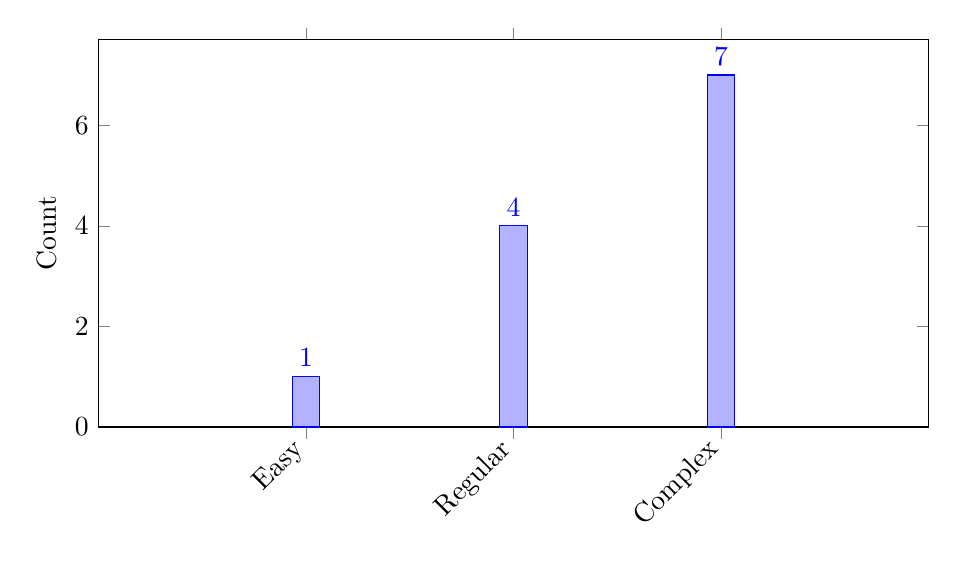
\begin{tikzpicture}
							\begin{axis}[
								ybar,
								width=\textwidth,
								height=6.5cm,
								symbolic x coords={Easy, Regular, Complex},
								xtick=data,
								ylabel={Count},
								%title={Monitoring Process of Students},
								ymin=0,
								nodes near coords,
								enlarge x limits=0.5,
								%title={Monitoring Process of Students},
								x tick label style={rotate=45, anchor=east} % Rotar etiquetas
								]
								\addplot coordinates {(Easy, 1) (Regular, 4) (Complex, 7)};
							\end{axis}
						\end{tikzpicture}
						\subcaption{Easiness of the monitoring process.}
						\label{fig:monitoring-process}
					\end{minipage}
					\vspace{5mm}
					\begin{minipage}{0.45\textwidth}
						\centering
						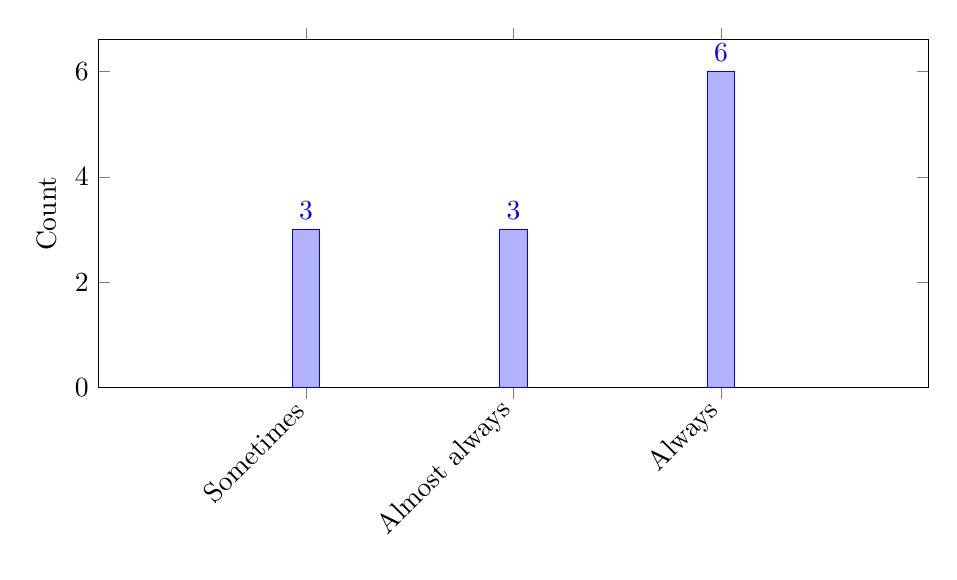
\begin{tikzpicture}
							\begin{axis}[
								ybar,
								width=\textwidth,
								height=6cm,
								symbolic x coords={Sometimes, Almost always, Always},
								xtick=data,
								ylabel={Count},
								ymin=0,
								nodes near coords,
								enlarge x limits=0.5,
								%title={Frequency of Monitoring Students},
								x tick label style={rotate=45, anchor=east} % Rotar etiquetas
								]
								\addplot coordinates {(Sometimes, 3) (Almost always, 3) (Always, 6)};
							\end{axis}
							%\label{fig:monitoring-frequency}
						\end{tikzpicture}
						\subcaption{Monitoring frequency.}
						\label{fig:monitoring-frequency}
					\end{minipage}
					\begin{minipage}{0.45\textwidth}
						\centering
						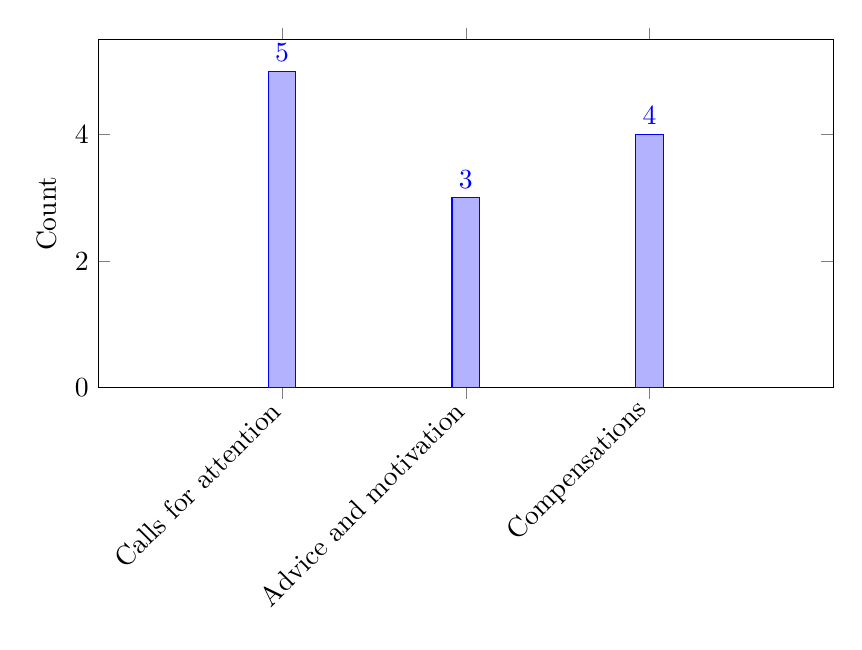
\begin{tikzpicture}
							\begin{axis}[
								ybar,
								height=6cm,
								width=0.9\textwidth,
								symbolic x coords={Calls for attention, Advice and motivation, Compensations},
								xtick=data,
								ylabel={Count},
								ymin=0,
								nodes near coords,
								enlarge x limits=0.5,
								%title={Strategies to Achieve Concentration},
								x tick label style={rotate=45, anchor=east} % Rotar etiquetas
								]
								\addplot coordinates {(Calls for attention, 5) (Advice and motivation, 3) (Compensations, 4)};
							\end{axis}
							%\label{fig:concentration-strategies}
						\end{tikzpicture}
						\subcaption{Strategies to achieve concentration.}
						\label{fig:concentration-strategies}
					\end{minipage}
					\caption{Results of questions asked to parents regarding the monitoring process of their elementary school children while doing homework.}
					\label{fig:previous-questions}
				\end{figure}

			\subsubsection{Tasks for Participant Users}
				The tasks that the tutors performed during the evaluation were as follows:
				
				\begin{enumerate}
					\item Connect the Torddis device to the power supply and place it on the desk where the child will be sitting to perform a task.
					\item Create a tutor user account in the mobile application.
					\item Log in to the mobile application.
					\item Register the child to be monitored.
					\item Register the Torddis device with the mobile application using the IP address provided on a label attached to the device.
					\item Perform facial training for the registered child.
					\item Enable and/or disable the objects to be monitored in the corresponding section of the mobile application.
					\item Assign a task to the child while being monitored by the Torddis device: colour a mandala.
					\item Activate the recognition of each distraction parameter in the monitoring section of the mobile application.
					\item Leave the child alone, without the presence of an adult, for 6 minutes.
					\item Enable and/or disable video transmission from the Torddis device.
					\item Navigate through the history of the distraction parameters monitored in the child.
					\item Visualize a report with charts depicting the distraction parameters detected for the monitored child.
				\end{enumerate}

			\subsubsection{Results of the System Usability Scale Questionnaire}
				The results analysed in this section correspond to the responses from the SUS questionnaire (see Appendix \ref{Appendix:LikertScale}) provided to the 12 tutors. After tabulating the obtained data, Figure \ref{fig:sus-questionnaire} shows that the mean of the collected data is 81.46\% with a standard deviation of 11.65. According to the adjectives (Worst imaginable, Poor, OK, Good, Excellent, Best imaginable) proposed by Bangor et al. \cite{Bangor2008AnEmpirical} to qualitatively assess the usability of a system based on the achieved mean, it is evident that Torddis has a ``Good'' usability level according to the evaluated tutors.
				
				\begin{figure}[hbt!]
					\centering
					\begin{tikzpicture}
						\begin{axis}[
							scatter/classes={
								a={mark=*,blue}
							},
							width=12cm,
							height=8cm,
							xlabel={Participant},
							ylabel={Evaluation},
							ymin=40, ymax=100,
							xmin=0, xmax=13,
							xtick={1,2,3,4,5,6,7,8,9,10,11,12},
							xticklabels={1,2,3,4,5,6,7,8,9,10,11,12},
							ytick={40,60,80,100},
							nodes near coords,
							every node near coord/.append style={font=\footnotesize, /pgf/number format/fixed},
							%title={SUS Questionnaire Data by Tutor},
							legend style={at={(0.5,-0.15)}, anchor=north, legend columns=-1},
							enlarge x limits=0.05,
							]
							\addplot[
							scatter,
							only marks,
							scatter src=explicit symbolic,
							visualization depends on=\thisrow{Evaluation} \as \label
							] table[meta=class,x=Participant,y=Evaluation] {
								Participant Evaluation class
								1 90.00 90.00
								2 95.00 95.00
								3 72.50 72.50
								4 60.00 60.00
								5 85.00 85.00
								6 67.50 67.50
								7 92.50 92.50
								8 67.50 67.50
								9 82.50 82.50
								10 85.00 85.00
								11 92.50 92.50
								12 87.50 87.50
							};
							
							% Línea de promedio
							\addplot [
							color=orange,
							thick,
							mark=none
							] coordinates {(0,\average) (13,\average)};
							
							% Línea de desviación estándar superior
							\addplot [
							color=orange,
							thick,
							dashed,
							mark=none
							] coordinates {(0,\upperlimit) (13,\upperlimit)};
							
							% Línea de desviación estándar inferior
							\addplot [
							color=orange,
							thick,
							dashed,
							mark=none
							] coordinates {(0,\lowerlimit) (13,\lowerlimit)};
							
							\legend{Participant, Average SUS, Std Dev}
						\end{axis}
					\end{tikzpicture}
					\caption{SUS questionnaire data by tutor with average evaluation and standard deviation.}
					\label{fig:sus-questionnaire}
				\end{figure}
	
			\subsubsection{Results of the Open-Ended Questions Questionnaire}
				At the end of the SUS questionnaire, the tutors answered 8 open-ended questions (see Appendix \ref{Appendix:OpenQuestions}) to provide their personal opinions.
				
				The first question asked was ``What is your overall opinion of the system?'', to which some tutors responded that it supports the students' concentration, and others said that it has a pleasant design. The results are shown in Figure \ref{fig:AboutTorddis}. The second open-ended question that the tutors answered was ``Did you find the sounds and/or lights that Torddis uses to be to your liking?''. Most tutors presented a  favourable opinion to this question since they believe that the light alerts help keep the student awake, and they are satisfied with the sound alarms (see Figure \ref{fig:SoundAndLigth}).
				
				\begin{figure}[hbt!]
					\centering
					\begin{minipage}{0.45\textwidth}
						\centering
						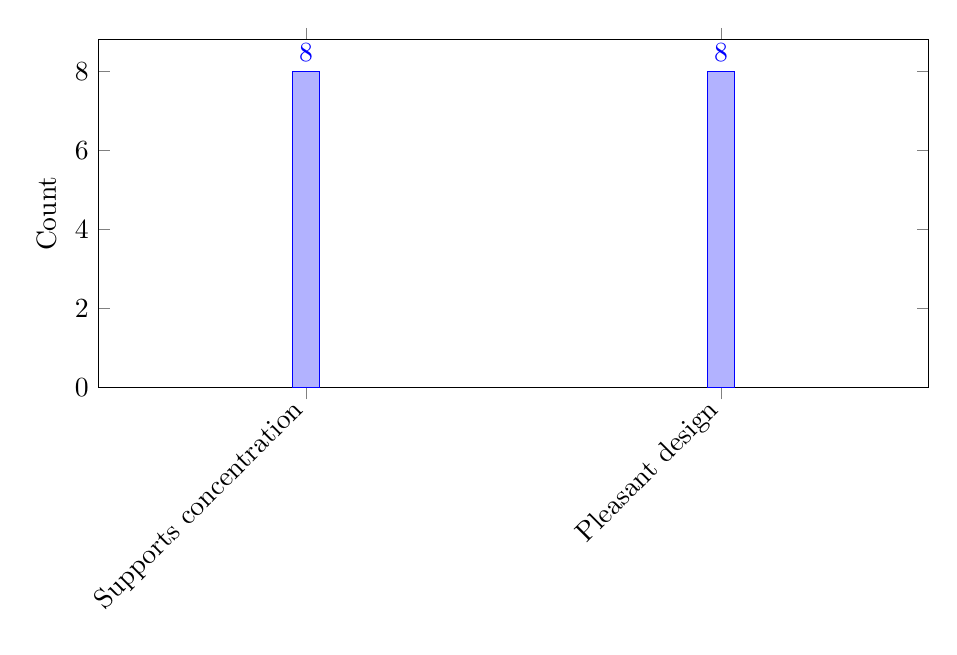
\begin{tikzpicture}
							\begin{axis}[
								ybar,
								width=\textwidth,
								height=6cm,
								symbolic x coords={Supports concentration, Pleasant design},
								xtick=data,
								ylabel={Count},
								%title={Monitoring Process of Students},
								ymin=0,
								nodes near coords,
								enlarge x limits=0.5,
								%title={Monitoring Process of Students},
								x tick label style={rotate=45, anchor=east} % Rotar etiquetas
								]
								\addplot coordinates {(Supports concentration, 8) (Pleasant design, 8)};
							\end{axis}
						\end{tikzpicture}
						\subcaption{Overall opinion about the Torddis system.}
						\label{fig:AboutTorddis}
					\end{minipage}
					\vspace{5mm}
					\begin{minipage}{0.45\textwidth}
						\centering
						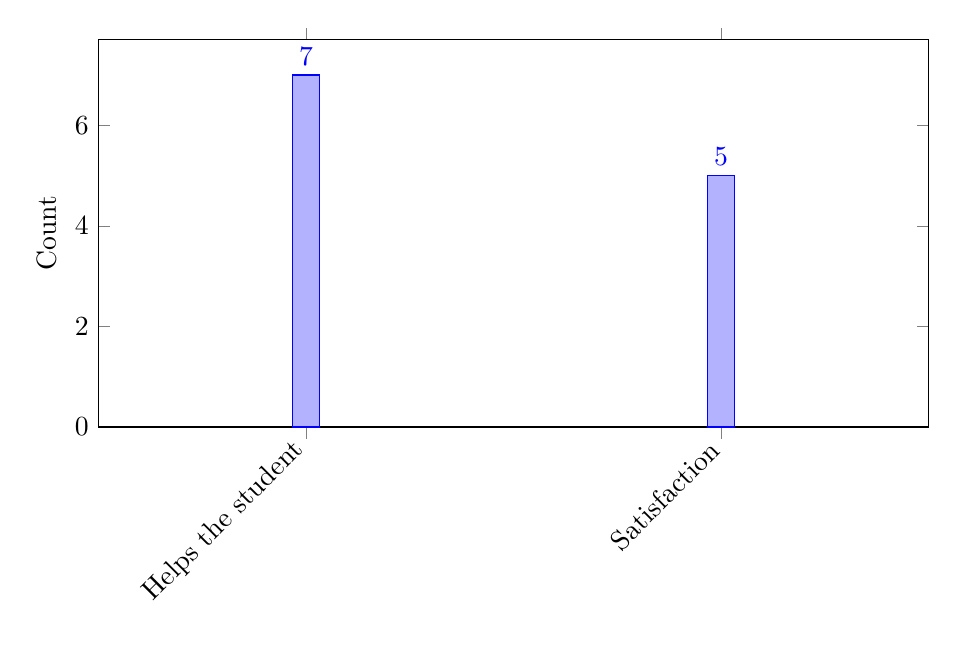
\begin{tikzpicture}
							\begin{axis}[
								ybar,
								width=\textwidth,
								height=6.5cm,
								symbolic x coords={Helps the student,Satisfaction},
								xtick=data,
								ylabel={Count},
								ymin=0,
								nodes near coords,
								enlarge x limits=0.5,
								%title={Frequency of Monitoring Students},
								x tick label style={rotate=45, anchor=east} % Rotar etiquetas
								]
								\addplot coordinates {(Helps the student, 7) (Satisfaction, 5)};
							\end{axis}
							%\label{fig:monitoring-frequency}
						\end{tikzpicture}
						\subcaption{Sound and light alerts of the system.}
						\label{fig:SoundAndLigth}
					\end{minipage}
					%\vspace{5mm}
					\begin{minipage}{0.45\textwidth}
						\centering
						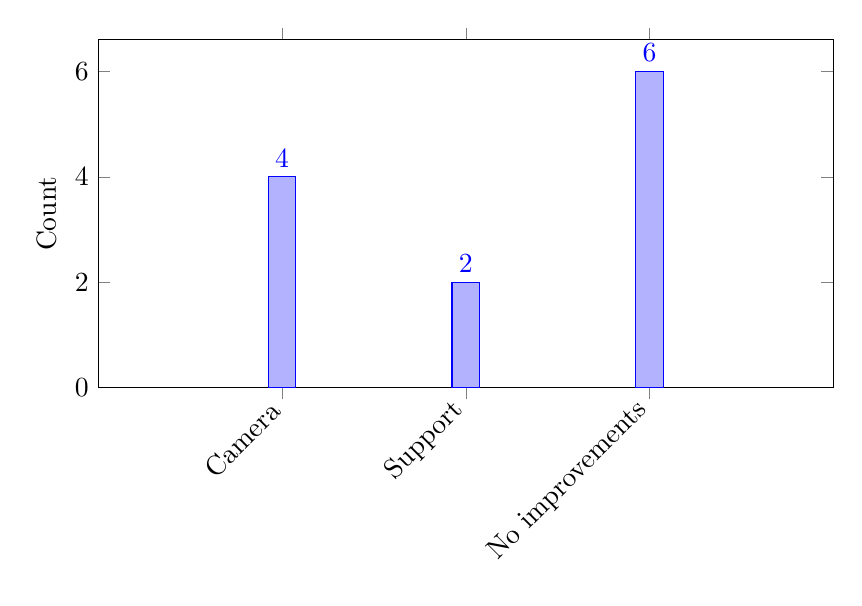
\begin{tikzpicture}
							\begin{axis}[
								ybar,
								height=6cm,
								width=0.9\textwidth,
								symbolic x coords={Camera, Support, No improvements},
								xtick=data,
								ylabel={Count},
								ymin=0,
								nodes near coords,
								enlarge x limits=0.5,
								%title={Strategies to Achieve Concentration},
								x tick label style={rotate=45, anchor=east} % Rotar etiquetas
								]
								\addplot coordinates {(Camera, 4) (Support, 2) (No improvements, 6)};
							\end{axis}
							%\label{fig:concentration-strategies}
						\end{tikzpicture}
						\subcaption{Suggestions for system improvements.}
						\label{fig:Improvements}
					\end{minipage}
					%\vspace{5mm}
					\begin{minipage}{0.45\textwidth}
						\centering
						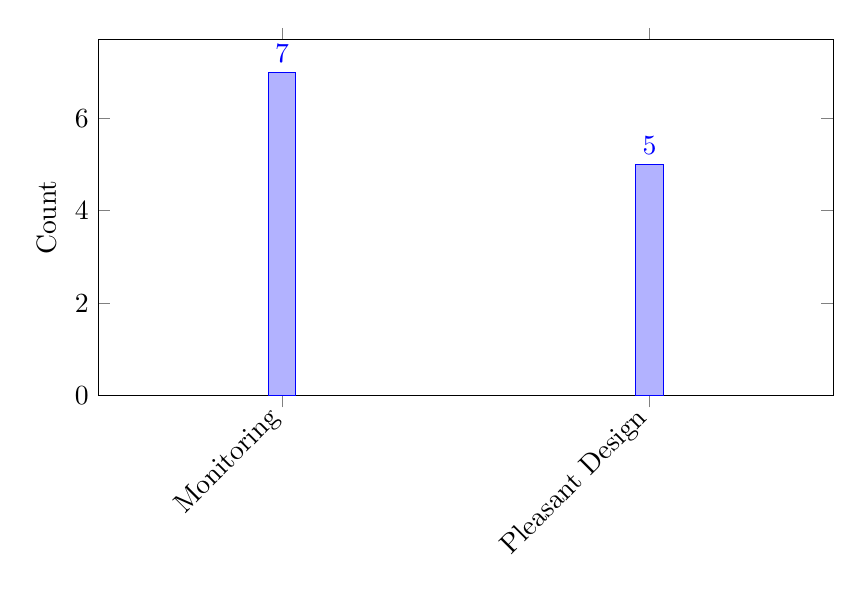
\begin{tikzpicture}
							\begin{axis}[
								ybar,
								height=6.1cm,
								width=0.9\textwidth,
								symbolic x coords={Monitoring, Pleasant Design},
								xtick=data,
								ylabel={Count},
								ymin=0,
								nodes near coords,
								enlarge x limits=0.5,
								%title={Strategies to Achieve Concentration},
								x tick label style={rotate=45, anchor=east} % Rotar etiquetas
								]
								\addplot coordinates {(Monitoring, 7) (Pleasant Design, 5)};
							\end{axis}
							%\label{fig:concentration-strategies}
						\end{tikzpicture}
						\subcaption{Reasons to recommend the system.}
						\label{fig:ReasonsRecomend}
					\end{minipage}
					\caption{Results of questions asked to parents regarding the monitoring process of their elementary school children using Torddis while doing homework.}
					\label{fig:AnswerOfOpenQuestion}
				\end{figure}
				
				In questions 3 (``Do you like the design of the Torddis mobile application? Why?''), 4 (``Is the way your child's distraction monitoring data is visualised in the Torddis mobile application adequate? Why?''), 5 (``Do you think this system would help improve your child's concentration and keep you informed when they are doing their schoolwork? Why?''), and 7 (``Would you be willing to continue using the Torddis system?''), all tutors expressed positive feedback. They stated that they liked the design of the mobile application views, highlighted the history data organization and the report charts, confirmed that the prototype system effectively supports children's concentration by keeping them informed when the child is distracted, and indicated their willingness to continue using the Torddis system.
				
				Question 6 intended to gather information indicating the improvements that could be made to Torddis. The feedback obtained includes using a higher quality camera and improving the support on which the camera  is mounted. However, a high percentage of users mentioned that the device does not need any further improvements. These results are shown in Figure \ref{fig:Improvements}. Meanwhile, question 8 gathered the reasons why the Torddis evaluators would recommend using this system for monitoring students during their school activities. Figure \ref{fig:ReasonsRecomend} shows the reasons mentioned by the tutors, including  that it helps them in monitoring their students and its pleasant design.

	\section{Conclusions}
	\label{seccion:Cinco}
		The Torddis prototype system has proven to be an effective and well-received tool for monitoring and improving student concentration during their school activities. Evaluations, including functional tests and usability questionnaires, revealed that the system meets the expected technical requirements and is highly appreciated by end-users, namely the tutors.
		
		The analysis of demographic and monitoring data indicates that Torddis significantly impacts managing children's distraction, providing tutors with a valuable tool to keep students focused on their tasks. The high score in the SUS usability questionnaire reinforces the perception that the system is easy to use and effective in its purpose.
		
		The Torddis person recognition system is efficient, with a 92.86\% success rate and an average recognition time of approximately 0.81 seconds, demonstrating solid performance under test conditions. Similarly, the facial expression recognition system shows a 92.86\% success rate with an average recognition time of approximately 1.36 seconds, highlighting its quick response times and reliability. The sleep presence recognition system is reasonably efficient, achieving an 85.71\% success rate and an average recognition time of approximately 3.43 seconds, indicating adequate performance.
		
		The distractor object recognition system, with a 78.57\% success rate and an average recognition time of approximately 2.33 seconds, performs adequately under test conditions.
		
		Additionally, feedback from open-ended questions shows strong support for the system's design and functionality, with valuable suggestions for future developments. Tutors highlighted the importance of visual and auditory alerts to keep students alert and the convenience of the system's configuration and monitoring options.
		
		In conclusion, Torddis has exceeded expectations in terms of functionality and usability, proving to be a viable and effective solution for maintaining student concentration in learning environments. The success of this project underscores the importance of technological innovation in education and paves the way for future improvements and expansions of the system.

	\section*{Acknowledgements}
	
	This research work has been supported by the grant PID2022-139297OB-I00, funded by MICIU/AEI/10.13039/ 501100011033 and by ERDF/EU.

	\printcredits
	
	\bibliographystyle{cas-model2-names}

	% Loading bibliography database
	\bibliography{torddisC&E-refs}
	
	\clearpage
	
	\appendix
	\section{Informed Consent} \label{Appendix:InformedConsent}
	Dear Participant,
	
	The purpose of this document is to provide you with the necessary information to decide whether or not to participate in the project titled "Internet of Things-based system for monitoring children's distraction during their academic activities at home", conducted under the direction of Professor Gleiston Cicerón Guerrero Ulloa MDS.
	
	Participation involves using the system provided as directed by the researchers. You will be required to sit in a specific place to use a mobile application. Meanwhile, your child will be monitored by an intelligent device called "Torddis" while performing a specific task directed by the researchers. The participation time is approximately 30 minutes, depending on each participant. These activities will be carried out in one of the researchers' homes.
	
	The information obtained through this study will be kept strictly confidential, and your names will not be used. You have the right to withdraw consent for participation at any time. The study does not involve any risk to you, nor will you receive any compensation. If you have any questions about this project, you can contact us at gguerrero@uteq.edu.ec.
	
	\vspace{0.5cm}
	\noindent\rule{3.65cm}{0.4pt} \hspace{1.1cm} \rule{4cm}{0.4pt} \hspace{1.1cm} \rule{4.2cm}{0.4pt}\\
	Carlos Almeida-Dueñas \hspace{2cm} John Plazarte-Suárez \hspace{2cm} Gleiston Guerrero-Ulloa
	
	After reading the procedure described above, having the researchers explain the procedure, and answering any questions, the participant (undersigned) voluntarily gives their consent to participate in this study.
	
	\vspace{0.5cm}
	\noindent
	Participant: \_\_\_\_\_\_\_\_\_\_\_\_\_\_\_\_\_\_\_\_\_\_\_\_\_\_\_\_\_\_\_\_\_\_\_\_
	Signature: \_\_\_\_\_\_\_\_\_\_\_\_\_\_\_\_\_\_\_\_\_\_\_\_
	Date: \_\_\_\_\_\_\_\_\_\_

	\clearpage
	\section[\appendixname~\thesection]{Demographic Survey} \label{Appendix:DemographicSurvey}
	\vspace{12pt}
	\noindent
	\textbf{1. Full Name: \_\_\_\_\_\_\_\_\_\_\_\_\_\_\_\_\_\_\_\_\_\_\_\_\_\_\_\_\_\_\_\_\_\_\_\_\_\_\_\_\_\_\_\_\_}
	
	\vspace{12pt}
	\noindent
	\textbf{2. Age: \_\_\_\_\_\_\_\_\_\_}
	
	\vspace{12pt}
	\noindent				
	\textbf{3. Level of Education:}
	
	\begin{itemize}
		\item No education ( )
		\item Primary ( )
		\item Secondary ( )
		\item Higher ( )
	\end{itemize}
	
	\noindent
	\textbf{4. Gender:}
	
	\begin{itemize}
		\item Male ( )
		\item Female ( )
		\item Other ( )
	\end{itemize}
	
	%\vspace{12pt.}
	\noindent
	\textbf{5. How has your experience been as a parent in monitoring your child's distractions while they are doing their schoolwork?}
	
	\begin{itemize}
		\item Easy ( )
		\item Regular ( )
		\item Complex ( )
		\item Very complex ( )
	\end{itemize}
	
	%\vspace{12pt.}
	\noindent
	\textbf{6. How often do you monitor your child's school activities?}
	
	\begin{itemize}
		\item Never ( )
		\item Sometimes ( )
		\item Almost always ( )
		\item Always ( )
	\end{itemize}
	
	%\vspace{12pt.}
	\noindent
	\textbf{7. What strategies have you implemented to improve your child's concentration during their homework?}
	
	\vspace{12pt}
	\noindent
	\rule{\textwidth}{1pt}
	
	\vspace{12pt}
	\noindent
	\rule{\textwidth}{1pt}
	
	\clearpage
	\section[\appendixname~\thesection]{SUS Questionnaire}
	\label{Appendix:SUSQuestionarie}
	
	
	\subsection[\appendixname~\thesection]{Questionnaire Likert Scale}
	\label{Appendix:LikertScale}
	The questions from the SUS questionnaire using the Likert scale are shown in Table \ref{tab:SUSQuestion}.
	
	\begin{table}[bt!]
		\caption{SUS Questionnaire \label{tab:SUSQuestion}}
		\centering
		\begin{tabular}{|p{10cm}|c|c|c|c|c|}
			\hline
			\textbf{Questions} & 1 & 2 & 3 & 4 & 5 \\
			\hline
			1. I would like to use the Torddis system frequently. & & & & & \\
			\hline
			2. I found the system unnecessarily complex. & & & & & \\
			\hline
			3. I thought the system was easy to use. & & & & & \\
			\hline
			4. I would need the support of a technician/teacher to use the system. & & & & & \\
			\hline
			5. I found the various functions of the system were well integrated (constituted a whole). & & & & & \\
			\hline
			6. I thought there were too many inconsistencies in the system. & & & & & \\
			\hline
			7. I imagine most people would learn to use the system quickly. & & & & & \\
			\hline
			8. I found the system very difficult to use. & & & & & \\
			\hline
			9. I felt very confident/comfortable using the system. & & & & & \\
			\hline
			10. I need to learn a lot of things before I can use the system. & & & & & \\
			\hline
		\end{tabular}
	\end{table}
	
	\subsection[\appendixname~\thesection]{Open Questions of SUS Questionnaire}
	\label{Appendix:OpenQuestions}
	The open questions of the SUS questionnaire are shown in Table \ref{tab:OpenQuestion}.
	\begin{table}[bt!]
		\centering
		\caption{Open Questions of SUS Questionnaire \label{tab:OpenQuestion}}
		\begin{tabularx}{\textwidth}{c X }
			\toprule
			\textbf{No.} & \textbf{Question} \\
			\midrule
			1 & In general, what is your opinion of the system? \\
			2 & Did you like the sounds and/or lights that the Torddis device contains? Please answer yes or no, and provide the reason. \\
			3 & Did you like the screen design of the Torddis mobile application? Please answer yes or no, and provide the reason. \\
			4 & Do you find the way the distraction monitoring data of your child is visualised in the Torddis mobile application to be adequate? Please answer yes or no, and provide suggestions. \\
			5 & Do you think this system would help improve your child's concentration and keep you informed when they are distracted? Please answer yes or no, and provide the reason. \\
			6 & Do you think there is anything that should be improved in the Torddis system (Device and Mobile Application)? If so, what? \\
			7 & Would you be willing to continue using the Torddis system? Please answer yes or no, and provide the reason. \\
			8 & Would you recommend this system to other people interested in monitoring children's distraction while doing schoolwork? Please answer yes or no, and provide the reason. \\ \bottomrule
		\end{tabularx}
	\end{table}
\end{document}

